\documentclass{article}

% if you need to pass options to natbib, use, e.g.:
%     \PassOptionsToPackage{numbers, compress}{natbib}
% before loading neurips_2020

% ready for submission
% \usepackage{neurips_2020}

% to compile a preprint version, e.g., for submission to arXiv, add add the
% [preprint] option:
%     \usepackage[preprint]{neurips_2020}

% to compile a camera-ready version, add the [final] option, e.g.:
%     \usepackage[final]{neurips_2020}

% to avoid loading the natbib package, add option nonatbib:

\usepackage[nonatbib]{neurips_2020}

\usepackage[utf8]{inputenc} % allow utf-8 input
\usepackage[T1]{fontenc}    % use 8-bit T1 fonts
\usepackage{hyperref}       % hyperlinks
\usepackage{url}            % simple URL typesetting
\usepackage{booktabs}       % professional-quality tables
\usepackage{amsfonts}       % blackboard math symbols
\usepackage{nicefrac}       % compact symbols for 1/2, etc.
\usepackage{microtype}      % microtypography

\usepackage{amsfonts}
\usepackage{bm}
\usepackage{tikz}
\usetikzlibrary{bayesnet}
\usetikzlibrary{arrows}
\usepackage{color}
\usepackage{graphicx}
\usepackage{caption}
\usepackage{subcaption}
\usetikzlibrary{backgrounds}
\usepackage{multirow}
\usepackage{algorithm}
\usepackage{algpseudocode}
\usepackage{amsthm}
\usepackage{mathtools}
\usepackage{wrapfig}
\usetikzlibrary{arrows.meta}

\newcommand{\een}{\mathbb{1}}
\newcommand{\vX}{\mathbf{X}}
\newcommand{\vx}{\mathbf{x}}
\newcommand{\vq}{\mathbf{q}}
\newcommand{\vf}{\mathbf{f}}
\newcommand{\ve}{\bm{\epsilon}}
\newcommand{\expectation}{\mathbb{E}}
\newcommand{\contribution}{{\phi}}
\newcommand{\val}{{v}}
\newcommand{\dodo}{\mathit{do}}
\newcommand{\ldo}[1]{\dodo(X_{#1} = x_{#1})}
\newcommand{\lvdo}[1]{\dodo(\vX_{#1} = \vx_{#1})}
\newcommand{\sdo}[1]{\hat{x}_{#1}}
\newcommand{\svdo}[1]{\hat{\vx}_{#1}}
\newcommand{\pa}{\mathop{\textit{pa}}}
\newcommand{\spa}{\mathop{\textit{\scriptsize pa}}}
\newcommand{\perm}{\pi}
\newcommand{\actcont}{\contribution^{\mbox{\scriptsize active}}}
\newcommand{\passcont}{\contribution^{\mbox{\scriptsize passive}}}
\newcommand{\operator}{\mathit{op}}
\newcommand{\sop}[1]{\operator(x_{#1})}
\newcommand{\svop}[1]{\operator(\vx_{#1})}
\newcommand{\lop}[1]{\operator(X_{#1} = x_{#1})}
\newcommand{\lvop}[1]{\operator(\vX_{#1} = \vx_{#1})}
\newcommand{\allfeatures}{{N}}
\newcommand{\bx}{\bar{x}}
\newcommand{\tx}{\tilde{x}}
\newcommand{\hx}{\hat{x}}
\newcommand{\allmeans}{{\cal X}}
\newcommand{\diagbeta}{{\cal B}}
\newcommand{\mapmat}{{\cal M}}
\newcommand{\contmat}{{\cal C}}
\newcommand{\onder}[2]{{#1}_{\mbox{\scriptsize #2}}}
\newcommand{\boven}[2]{#1^{\mbox{\scriptsize #2}}}
\newcommand{\isequal}{\hspace*{-2.5mm} & = & \hspace*{-2.5mm}}
\newcommand{\chaincomponents}{{\cal T}}
\newcommand{\isequaldo}[1]{\hspace*{-2.5mm} & \overset{(#1)}{=} & \hspace*{-2.5mm}}
\newcommand{\Spre}{\underline{S}}
\newcommand{\Spost}{\bar{S}}

\newcommand{\comment}[1]{{\color{red} #1}}


\newtheorem{theorem}{Theorem}
\newtheorem{corollary}[theorem]{Corollary}

\title{Causal Shapley Values: Exploiting Causal Knowledge to Explain Individual Predictions of Complex Models} 

% The \author macro works with any number of authors. There are two commands
% used to separate the names and addresses of multiple authors: \And and \AND.
%
% Using \And between authors leaves it to LaTeX to determine where to break the
% lines. Using \AND forces a line break at that point. So, if LaTeX puts 3 of 4
% authors names on the first line, and the last on the second line, try using
% \AND instead of \And before the third author name.

\author{%
  Pietje Puk\\
  Radboud University
  Institute for Computing and Information Sciences\\
  Nijmegen, The Netherlands \\
  \texttt{pietje.puk@ru.nl} \\
  % examples of more authors
  % \And
  % Coauthor \\
  % Affiliation \\
  % Address \\
  % \texttt{email} \\
  % \AND
  % Coauthor \\
  % Affiliation \\
  % Address \\
  % \texttt{email} \\
  % \And
  % Coauthor \\
  % Affiliation \\
  % Address \\
  % \texttt{email} \\
  % \And
  % Coauthor \\
  % Affiliation \\
  % Address \\
  % \texttt{email} \\
}

\begin{document}

\maketitle

\begin{abstract}
Shapley values underlie one of the most popular model-agnostic methods within explainable artificial intelligence. These values are designed to attribute the difference between a model's prediction and an average baseline to the different features used as input to the model. Being based on solid game-theoretic principles, Shapley values uniquely satisfy several desirable properties, which is why they are increasingly used to explain the predictions of possibly complex and highly non-linear machine learning models. Shapley values are well calibrated to a user’s intuition when features are independent, but may lead to undesirable, counter-intuitive explanations when the independence assumption is violated.

In this paper, we propose a novel framework for computing Shapley values that generalizes recent work that aims to circumvent the independence assumption. By employing Pearl's \textit{do}-calculus, we show how these `causal' Shapley values can be derived for general causal graphs without sacrificing any of their desirable properties. Moreover, causal Shapley values enable us to separate the contribution of direct and indirect effects. We provide a practical implementation for computing causal Shapley values based on causal chain graphs when only partial information is available and illustrate their utility on a real-world example.
\end{abstract}


%The \LaTeX{} style file contains three optional arguments: \verb+final+, which creates a camera-ready copy, \verb+preprint+, which creates a preprint for submission to, e.g., arXiv, and \verb+nonatbib+, which will not load the \verb+natbib+ package for you in case of package clash.

%If you wish to post a preprint of your work online, e.g., on arXiv, using the NeurIPS style, please use the \verb+preprint+ option. This will create a nonanonymized version of your work with the text ``Preprint. Work in progress.'' in the footer. This version may be distributed as you see fit. Please \textbf{do not} use the \verb+final+ option, which should \textbf{only} be used for papers accepted to NeurIPS.

%At submission time, please omit the \verb+final+ and \verb+preprint+options. This will anonymize your submission and add line numbers to aid review. Please do \emph{not} refer to these line numbers in your paper as they will be removed during generation of camera-ready copies.


%There is also a \verb+\paragraph+ command available, which sets the heading in bold, flush left, and inline with the text, with the heading followed by 1\,em of space.

%The \verb+natbib+ package will be loaded for you by default.  Citations may be author/year or numeric, as long as you maintain internal consistency.  As to the format of the references themselves, any style is acceptable as long as it is used consistently.

%Of note is the command \verb+\citet+, which produces citations appropriate for use in inline text.  For example,
%\begin{verbatim}
%   \citet{hasselmo} investigated\dots
%\end{verbatim}
%produces
%\begin{quote}
%  Hasselmo, et al.\ (1995) investigated\dots
%\end{quote}

%If you wish to load the \verb+natbib+ package with options, you may add the following before loading the \verb+neurips_2020+ package:
%\begin{verbatim}
%   \PassOptionsToPackage{options}{natbib}
%\end{verbatim}

%If \verb+natbib+ clashes with another package you load, you can add the optional
%argument \verb+nonatbib+ when loading the style file:
%\begin{verbatim}
%   \usepackage[nonatbib]{neurips_2020}
%\end{verbatim}

%Footnotes should be used sparingly.  If you do require a footnote, indicate footnotes with a number\footnote{Sample of the first footnote.} in the text. Place the footnotes at the bottom of the page on which they appear. Precede the footnote with a horizontal rule of 2~inches (12~picas).
%
%Note that footnotes are properly typeset \emph{after} punctuation
%marks.\footnote{As in this example.}


%Note that publication-quality tables \emph{do not contain vertical rules.} We strongly suggest the use of the \verb+booktabs+ package, which allows for typesetting high-quality, professional tables:
%\begin{center}
%  \url{https://www.ctan.org/pkg/booktabs}
%\end{center}
%This package was used to typeset Table~\ref{sample-table}.
%
%\begin{table}
%  \caption{Sample table title}
%  \label{sample-table}
%  \centering
%  \begin{tabular}{lll}
%    \toprule
%    \multicolumn{2}{c}{Part}                   \\
%    \cmidrule(r){1-2}
%    Name     & Description     & Size ($\mu$m) \\
%    \midrule
%    Dendrite & Input terminal  & $\sim$100     \\
%    Axon     & Output terminal & $\sim$10      \\
%    Soma     & Cell body       & up to $10^6$  \\
%    \bottomrule
%  \end{tabular}
%\end{table}

%Please prepare submission files with paper size ``US Letter,'' and not, for example, ``A4.''

%\begin{itemize}
%
%\item You should directly generate PDF files using \verb+pdflatex+.
%
%\item You can check which fonts a PDF files uses.  In Acrobat Reader, select the
%  menu Files$>$Document Properties$>$Fonts and select Show All Fonts. You can
%  also use the program \verb+pdffonts+ which comes with \verb+xpdf+ and is
%  available out-of-the-box on most Linux machines.
%
%\item The IEEE has recommendations for generating PDF files whose fonts are also
%  acceptable for NeurIPS. Please see
%  \url{http://www.emfield.org/icuwb2010/downloads/IEEE-PDF-SpecV32.pdf}
%
%\item \verb+xfig+ "patterned" shapes are implemented with bitmap fonts.  Use
%  "solid" shapes instead.
%
%\item The \verb+\bbold+ package almost always uses bitmap fonts.  You should use the equivalent AMS Fonts:
%\begin{verbatim}
%   \usepackage{amsfonts}
%\end{verbatim}
%followed by, e.g., \verb+\mathbb{R}+, \verb+\mathbb{N}+, or \verb+\mathbb{C}+
%for $\mathbb{R}$, $\mathbb{N}$ or $\mathbb{C}$.  You can also use the following
%workaround for reals, natural and complex:
%\begin{verbatim}
%   \newcommand{\RR}{I\!\!R} %real numbers
%   \newcommand{\Nat}{I\!\!N} %natural numbers
%   \newcommand{\CC}{I\!\!\!\!C} %complex numbers
%\end{verbatim}
%Note that \verb+amsfonts+ is automatically loaded by the \verb+amssymb+ package.
%
%\end{itemize}

%Most of the margin problems come from figures positioned by hand using \verb+\special+ or other commands. We suggest using the command
%\verb+\includegraphics+ from the \verb+graphicx+ package. Always specify the figure width as a multiple of the line width as in the example below:
%\begin{verbatim}
%   \usepackage[pdftex]{graphicx} ...
%   \includegraphics[width=0.8\linewidth]{myfile.pdf}
%\end{verbatim}
%See Section 4.4 in the graphics bundle documentation
%(\url{http://mirrors.ctan.org/macros/latex/required/graphics/grfguide.pdf})
%
%A number of width problems arise when \LaTeX{} cannot properly hyphenate a
%line. Please give LaTeX hyphenation hints using the \verb+\-+ command when
%necessary.





%Do {\bf not} include this section in the anonymized submission, only in the final paper. You can use the \texttt{ack} environment provided in the style file to autmoatically hide this section in the anonymized submission.
%\end{ack}

%\section*{References}
%
%References follow the acknowledgments. Use unnumbered first-level heading for the references. Any choice of citation style is acceptable as long as you are consistent. It is permissible to reduce the font size to \verb+small+ (9 point)
%when listing the references.
%{\bf Note that the Reference section does not count towards the eight pages of content that are allowed.}
%\medskip

%\small

\section{Introduction}

Complex machine learning models like deep neural networks and ensemble methods like random forest and gradient boosting machines may well outperform simpler approaches such as linear regression or single decision trees, but are noticeably harder to interpret. This can raise practical, ethical, and legal issues, most notably when applied in critical systems, e.g., for medical diagnosis or autonomous driving. The field of explainable AI aims to address these issues by enhancing the interpretability of complex machine learning models.

The Shapley-value approach has quickly become one of the most popular model-agnostic methods within explainable AI. It can provide local explanations, attributing changes in predictions for individual data points to the model's features, that can be combined to obtain better global understanding of the model structure~\cite{lundberg2020local}. Shapley values are based on a principled mathematical foundation~\cite{shapley1953value} and satisfy various desiderata (see also Section~\ref{sec:interpretation}). They have been applied for explaining statistical and machine learning models for quite some time, see e.g.,~\cite{lipovetsky2001analysis,vstrumbelj2014explaining}. Recent interests have been triggered by Lundberg and Lee's breakthrough paper~\cite{lundberg2017unified} that introduces efficient computational procedures and unifies Shapley values and other popular local model-agnostic approaches such as LIME~\cite{ribeiro2016should}.

Humans have a strong tendency to reason about their environment in causal terms~\cite{sloman2005causal}, where explanation and causation are intimately related: explanations often appeal to causes, and causal claims often answer questions about why or how something occurred~\cite{lombrozo2017causal}. The specific domain of causal responsibility studies how people attribute an effect to one or more causes, all of which may have contributed to the observed effect~\cite{sober1988apportioning}. Causal attributions by humans strongly depend on a subject's understanding of the generative model that explains how different causes lead to the effect, for which the relations between these causes are essential~\cite{gerstenberg2012noisy}.

%How much acceleration would there have been, if the gravitational force had acted, but the electrical force had been absent? How much acceleration would there have been, if the electrical force had acted, but the gravitational force had been absent?~\cite{sober1988apportioning}


%people compare what actually happened when the cause was present, with what they think would have happened in the absence of the cause~\cite{gerstenberg2012noisy}
%
%
%
%At its core ‘explainability’ is a causal notion. Humans have a strong tendency to reason in causal terms~\cite{sloman2005causal}, and explanations in causal terms tend to better align with a user's intuition. If a clinician asks ‘ok, but why does the algorithm predict a high risk of cancer for this patient’, she essentially asks for a rationale that gives insight into the effective relative contribution of each input feature to the target outcome prediction. 

Most explanation methods, however, tend to ignore such relations and act as if features are independent. Even so-called counterfactual approaches, that strongly rely on a causal intuition, make this simplifying assumption (e.g.,~\cite{wachter2017counterfactual}) and ignore that, in the real world, a change in one input feature may cause a change in another. This independence assumption also underlies early Shapley-based approaches, such as~\cite{vstrumbelj2014explaining,datta2016algorithmic}, and is made explicit as an approximation for computational reasons in~\cite{lundberg2017unified}. We will refer to these as {\em marginal} Shapley values.

%When applied to explain the predictions of a machine learning model, Shapley values consider the difference between the model's prediction when knowing all feature values and its baseline prediction when knowing none of the feature values and split this difference among the features that are used as input to the model. A crucial subroutine of the approach needs to compute or estimate the expected model output when some features are known, while others are dropped.
Aas et al.~\cite{aas2019explaining} argue and illustrate that marginal Shapley values may lead to incorrect explanations when features are highly correlated, motivating what we will refer to as {\em conditional} Shapley values. Janzing et al.~\cite{janzing2019feature}, following~\cite{datta2016algorithmic}, discuss a causal interpretation of Shapley values, in which they replace conventional conditioning by observation with conditioning by intervention, as in Pearl's {\em do}-calculus~\cite{pearl2012calculus}. This, somewhat surprisingly, leads them to conclude that marginal Shapley values are to be preferred over conditional ones. Their argument is also picked up by~\cite{lundberg2020local} when implementing interventional Tree SHAP. Frye et al.~\cite{frye2019asymmetric} propose {\em asymmetric} Shapley values as a way to incorporate causal knowledge by restricting the possible permutations of the features when computing the Shapley values to those consistent with a (partial) causal ordering. In line with~\cite{aas2019explaining}, they then apply conventional conditioning by observation to make sure that the explanations respect the data manifold.

%In this paper, we will follow~\cite{datta2016algorithmic,	janzing2019feature,lundberg2020local} in starting from an active interpretation of Shapley values, but show how the causal structure can be exploited to properly account for dependencies between features.
The main contributions of our paper are as follows.
(1)~We derive {\em causal} Shapley values that explain the total effect of features on the prediction, taking into account their causal relationships. This makes them principally different from marginal and conditional Shapley values. Compared to asymmetric Shapley values, causal Shapley values provide a more direct way to incorporate causal knowledge. (2)~Our method allows for further insights into feature relevance by separating out the total causal effect into a direct and indirect contribution. 
%where the `direct' aspect has a similar focus as the marginal Shapley values, and the `indirect' component puts more emphasis on the root cause contribution associated with asymmetric Shapley values.
%We extend the concept of Shapley values with the possibility to decompose feature attributions in direct and indirect effects.
(3)~Making use of causal chain graphs~\cite{lauritzen2002chain}, we propose a practical approach for computing causal Shapley values and illustrate this on a real-world example.

\section{A causal interpretation of Shapley values}
\label{sec:interpretation}

In this section, we will introduce our causal, interventional interpretation of Shapley values and contrast this to other approaches.
%We consider the standard supervised machine learning scenario, in which we are given examples of feature vectors $\vx$ with corresponding targets $y$, assumed to be drawn from an unknown distribution $P(Y|\vx)$. After training, we have access to a model $f(\vx)$, e.g., a deep neural network or an ensemble of trees, that can provide a prediction for every possible feature vector $\vx$. In most supervised learning applications, a successfully trained model approximates some (link) function of the expectation $\expectation[Y|x]$:
%\[
%f(\vx) \approx g(\expectation[Y|\vx]) \: ,
%\]
%with just the identity $g(z) = z$ for regression and for binary classification either the identity (as in~\cite{aas2019explaining}) or the logit $g(z) = \log (z/(1-z))$ (as in~\cite{lundberg2017unified}).
We assume that we are given a machine learning model $f(\cdot)$ that can generate predictions for any feature vector $\vx$. Our goal is to provide an explanation for an individual prediction $f(\vx)$, that takes into account the causal relationships between the features.

Attribution methods, with Shapley values as their most prominent example, provide a local explanation of individual predictions by attributing the difference between $f(\vx)$ and a baseline $f_0$ to the different features $i \in \allfeatures$ with $\allfeatures = \{1,\ldots,n\}$ and $n$ the number of features:
\begin{equation}
f(\vx) = f_0 + \sum_{i=1}^n \contribution_i \: ,
\label{eq:efficiency}
\end{equation}
where $\contribution_i$ is the contribution of feature $i$ to the prediction $f(\vx)$. For the baseline $f_0$ we will take the average prediction $f_0 = \expectation f(\vX)$ with expectation taken over the observed data distribution $P(\vX)$.
%, corresponding to not knowing any of the feature values.
Equation~(\ref{eq:efficiency}) is referred to as the {\em efficiency property}~\cite{shapley1953value}, which appears to be a sensible desideratum for any attribution method and we therefore take here as our starting point.

To go from knowing none of the feature values, as for $f_0$, to knowing all feature values, as for $f(\vx)$, we can add feature values one by one, actively setting the features to their values in a particular order $\perm$.
% Here we can think of (at least) two possible interpretations.
%\begin{description}
%	\item[Passive.] We interpret the feature vector $\vx$ as a passive observation. Feature values come in one after the other and the contribution of feature $i$ should reflect the difference in expected value of $f(\vX)$ after and before {\em observing} its feature value $x_i$.
%	\item[Active.] We interpret the feature vector $\vx$ as the result of an action. Feature values are imposed one after the other and the contribution of feature $i$ relates to the difference in expected value of $f(\vX)$ after and before {\em setting} its value to $x_i$.
%\end{description}
%Following the above reasoning,
We define the contribution of feature $i$ given permutation $\perm$ as the difference in value function before and after setting the feature to its value:
\begin{equation}
\contribution_i(\perm) = \val(\{j: j \preceq_\perm i\}) - \val(\{j: j \prec_\perm i\}) \: ,
\label{eq:contperm}
\end{equation}
with $j \prec_\perm i$ if $j$ precedes $i$ in the permutation $\perm$
%and $j \preceq_\perm i$ if $j$ precedes $i$ or is equal to $i$,
and where we choose the value function
\begin{equation}
\val(S) = \expectation \left[f(\vX) | \lvdo{S} \right] = \int d\vX_{\bar{S}} \: P(\vX_{\bar{S}}|\lvdo{S}) f(\vX_{\bar{S}},\vx_S) \: .
\label{eq:valuedef}
\end{equation}
Here $S$ is the subset of `in-coalition' indices with known feature values $\vx_S$. To compute the expectation, we average over the `out-of-coalition' or dropped features $\vX_{\bar{S}}$ with $\bar{S} = \allfeatures \setminus S$, the complement of $S$. To explicitly take into account that we actively {\em set} the features to their values, we condition `by intervention' 
%The operator $\operator()$ specifies how the distribution of the `out-of-coalition' features $\vX_{\bar{S}}$ depends on the `in-coalition' feature values $\vx_{S}$. For the passive interpretation, we set $\operator()$ to conventional conditioning by observation, yielding $P(\vX_{\bar{S}}|\vx_{S})$.
for which we resort to Pearl's \textit{do}-calculus~\cite{pearl1995causal}. In words, the contribution $\contribution_i(\perm)$ now measures the relevance of feature $i$ through the (average) prediction obtained if we actively set feature $i$ to its value $x_i$ compared to (the counterfactual situation of) not knowing its value.

Since the sum over features $i$ in~(\ref{eq:contperm}) is telescoping, the efficiency property~(\ref{eq:efficiency}) holds for any permutation $\perm$.
%\begin{eqnarray*}
%\sum_{i=1}^m \contribution_i(\perm) & = & \sum_{i=1}^m \left(
%\expectation \left[f(\vX) | \svop{\{j:\perm(j) \leq \perm(i)\}} \right] - \expectation \left[f(\vX) | \svop{\{j:\perm(j) < \perm(i)\}} \right] \right) \\
%& = & \sum_{i=1}^m \left(\expectation \left[f(\vX) | \svop{\{j:j \leq i\}} \right] - \expectation \left[f(\vX) | \svop{\{j:j < i\}} \right] \right) \\
%& = & \expectation \left[f(\vX) | \svop{\{j:j \leq m\}} \right] - \expectation \left[f(\vX) | \svop{\{j:j < 1\}} \right] \\
%& = & f(\vx) - \expectation [f(\vX)] \: .
%\end{eqnarray*}
Therefore, for any distribution over permutations $w(\perm)$ with $\sum_{\perm} w(\perm) = 1$, the contributions
\begin{equation}
\contribution_i = \sum_{\perm} w(\perm) \contribution_i(\perm)
\label{eq:shapperm}
\end{equation}
still satisfy~(\ref{eq:efficiency}). An obvious choice would be to take a uniform distribution $w(\perm) = 1/n!$. We then arrive at the standard formula for Shapley values (with shorthand $i$ for the singleton $\{i\}$):
\[
\contribution_i = \sum_{S \subseteq \allfeatures\setminus i} \frac{|S|! (n-|S|-1)!}{n!} \left[\val(S \cup i) - \val(S) \right] \: .
\]
Besides efficiency, the Shapley values uniquely satisfy three other desirable properties~\cite{shapley1953value}.
\begin{description}
	\item[Linearity:] for two value functions $\val_1$ and $\val_2$, we have $\contribution_i(\alpha_1 \val_1 + \alpha_2 \val_2) = \alpha_1 \contribution_i(\val_1) + \alpha_2 \contribution_i(\val_2)$. This guarantees that the Shapley value of a linear ensemble of models is a linear combination of the individual Shapley values.
	\item[Null player (dummy):] if $\val(S \cup i) = \val(S)$ for all $S \subseteq \allfeatures \setminus i$, then $\contribution_i = 0$. A feature that never contributes to the prediction (directly nor indirectly, see below) receives zero Shapley value.
	\item[Symmetry:] if $\val(S \cup i) = \val(S \cup j)$ for all  $S \subseteq \allfeatures \setminus \{i,j\}$, then $\contribution_i = \contribution_j$. Symmetry holds for marginal, conditional, and causal Shapley values.
\end{description}
Efficiency, linearity, and null player still hold for a non-uniform distribution of permutations as in~\cite{frye2019asymmetric}, but symmetry is then typically lost.

Replacing conditioning by intervention with conventional conditioning by observation, i.e., averaging over $P(\vX_{\bar{S}}|\vx_{S})$ instead of $P(\vX_{\bar{S}}|\lvdo{S})$ in~(\ref{eq:valuedef}), we arrive at the conditional Shapley values of~\cite{aas2019explaining,lundberg2018consistent}. A third option is to ignore the feature values $\vx_S$ and take the unconditional, marginal distribution $P(\vX_{\bar{S}})$, which leads to the marginal Shapley values.
%We will argue in Section~\ref{sec:toymodels} that causal Shapley values, computed through conditioning by intervention, are the only ones that can sensibly measure the total effect of an input feature on the model's prediction for general causal structures between the input features.
%Properties such as null player and symmetry are defined with reference to the value function or, equivalently, w.r.t.\ binary variables indicating for each feature whether it is `in-coalition' or `out-of-coalition', so not with respect to the function $f(\vx)$ itself as in~\cite{sundararajan2019many}. In the latter case, only marginal Shapley values satisfy the null player property, but are not even guaranteed to satisfy the symmetry property: even though $f(x_1,x_2) = f(x_2,x_1)$, for all possible values $x_1$ and $x_2$, we can get $\phi_1 \neq \phi_2$ when $P(x_1) \neq P(x_2)$. \comment{Remove?}

%To understand which interpretation and then also type of Shapley values to prefer, we go back to what $f(\vx)$ is actually supposed to represent: some function of the expectation of the target $Y$ given the features values $\vx$. When the features are potential causes of the target $Y$, we have $\expectation[Y|\vx] = \expectation[Y|\lvdo{}]$. In this case, causal Shapley values, providing an explanation in terms of actively setting features to their values, appear to be the most natural and informative choice, as we will also illustrate through examples in the next section. However, when the features are themselves mere consequences of the target $Y$, an active, interventional interpretation makes no sense, since then $\expectation[Y|\lvdo{}] = \expectation[Y] \neq \expectation[Y|\vx]$. As an example, $Y$ could represent the presence or absence of a disease and $\vx$ the outcome of clinical tests. It is perfectly fine to build a predictive model for the probability of the disease given test outcomes, but an explanation of how the prediction changes when we actively set a test outcome to its value makes no sense. When some features are causes of the target $Y$ and others consequences, we can consider actively setting the causes and passively observing the consequences. This more complicated setting is beyond the scope of the paper.

From the outset, our active, interventional interpretation of Shapley values appears to coincide with that in~\cite{datta2016algorithmic,janzing2019feature,lundberg2020local}. However, the construction in Janzing et al.~\cite{janzing2019feature} ignores any dependencies between the features in the real world, by formally distinguishing between true features (corresponding to one of the data points) and the features plugged as input into the model. This leads to the conclusion that, in our notation, $P(\vX_{\bar{S}}|\lvdo{S}) = P(\vX_{\bar{S}})$ for any subset $S$. As a result, any expectation under conditioning by intervention collapses to a marginal expectation and, in the interpretation of~\cite{datta2016algorithmic,janzing2019feature,lundberg2020local}, interventional Shapley values conveniently simplify to marginal Shapley values. As we will see below, marginal Shapley values can only represent direct effects, which makes that `root causes' with strong indirect effects (e.g.\ genetic markers) are ignored in the attribution, which is quite different from how humans tend to attribute causes~\cite{sober1988apportioning}.

%Although the chosen construction is technically correct, it then also appears to throw the baby out with the bathwater: the (then reduced to marginal) Shapley values by construction can only incorporate direct effects and fail to provide insight into the {\em total effect} of setting a feature to its value.

%Unlike~\cite{janzing2019feature}, we do not consider the function $f(\vX)$ to be just any technical input-output system, but assume that it has been trained to estimate the causal relationship between features $\vX$ and a target variable $Y$. In a typical machine learning scenario, a model trained on a set of examples relates to the expectation of the target variable given the input variables:
%\[
%f(\vx) \approx g(\expectation[Y|\vx]) \: ,
%\]
%with $g(\cdot)$ a link function, typically just the identity $g(z) = z$ for regression and the logit $g(z) = \log (z/(1-z))$ for binary classification. Assuming that the features $\vX$ can indeed be considered potential causes of the target variable $Y$, we have $\expectation[Y|\vX] = \expectation[Y|\lvdo{}]$. Note that this excludes models in which the target $Y$ is better viewed as a cause of (some) of the features.


%When all dependencies between features are the result of confounding,
%conditioning by intervention reduces to no conditioning at all, $P(\vX_{\bar{S}}|\lvdo{S}) = P(\vX_{\bar{S}})$ for any subset $S$, and causal Shapley values simplify to marginal Shapley values. However, as we will show in the next sections, when the features are causally related, for example, when one feature drives another or when dependencies between features are better explained through mutual interactions instead of through confounding, the argumentation for unconditional expectations breaks down.

%They make a case for using the marginal instead of the (observational) conditional distribution to compute the Shapley values when dependencies between features are due to confounding. This follows directly from our reasoning, since in models with no causal links between the features and any dependencies only due to confounding, conditioning by intervention reduces to the marginal distribution:

%\comment{Need to discuss~\cite{lundberg2020local}. It claims an intervential Tree SHAP and uses do-calculus notation. Writes ``interventional Tree SHAP (by the laws of causality) enforces an independence between the conditional set S and the set of remaining features $\bar{S}$ ($\vX_S \perp \vX_{\bar{S}}$)''. To be honest, I have no clue where their claim comes from, apart from a reference to Janzing\ldots}

When applied to incorporate causal knowledge, the asymmetric Shapley values introduced in~\cite{frye2019asymmetric} choose $w(\perm) \neq 0$ in~(\ref{eq:shapperm}) only for those permutations $\perm$ that are consistent with the causal structure between the features, i.e., are such that a known causal ancestor always precedes its descendants. In a strong causal chain now only the root cause gets all the credit, which is erring on the opposite side of the explanation spectrum compared to completely ignoring it.
%Asymmetric Shapley values provide somewhat of a mix between an active, interventional (incorporating causal structure into the allowed permutations) and passive, observational (conditioning by observation) approach.
This asymmetric idea can be considered orthogonal to the replacement of conditioning by observation with conditioning by intervention. We will therefore refer to the approach of~\cite{frye2019asymmetric} as {\em asymmetric conditional} Shapley values, to contrast them with {\em asymmetric causal} Shapley values that implement both ideas.

\section{Decomposing Shapley values into direct and indirect effects}

%Having a causal interpretation of Shapley values, we can decompose our explanation to reflect the contribution of direct and indirect effects.
Our causal interpretation allows us to distinguish between direct and indirect effects of each feature on a model's prediction. This is most easily seen by going back to the contribution $\contribution_i(\perm)$ for a permutation $\perm$ and feature $i$ in (\ref{eq:contperm}).
%that measures the difference in value function with and without adding $X_i$ to the `in-coalition' features.
%This addition has two effects: a direct effect because now we know the value of $x_i$ and an indirect effect because adding $\ldo{i}$ to the interventional set may change the distribution of the other features.
With shorthand notation $\Spre = \{j: j \prec_\perm i\}$ and $\Spost = \{j: j \succ_\perm i\}$, we can decompose the total effect for this permutation into a direct and an indirect effect:
\begin{eqnarray*}
	\contribution_i(\perm) \isequal
	%\val(\Spre \cup i) - \val(\Spre) \\ \isequal
	\expectation[f(\vX_{\Spost},\vx_{\Spre \cup i})|\lvdo{\Spre \cup i}] - \expectation[f(\vX_{\Spost \cup i},\vx_{\Spre})|\lvdo{\Spre}] ~~~~~~\mbox{(total effect)} \\
	\isequal \expectation[f(\vX_{\Spost},\vx_{\Spre \cup i})|\lvdo{\Spre}] - \expectation[f(\vX_{\Spost \cup i},\vx_{\Spre})|\lvdo{\Spre}] + ~~~~~~~\mbox{(direct effect)} \\
	&& \! \! \! \! \expectation[f(\vX_{\Spost},\vx_{\Spre \cup i})|\lvdo{\Spre \cup i}] - \expectation[f(\vX_{\Spost},\vx_{\Spre \cup i})|\lvdo{\Spre}] ~~~~\mbox{(indirect effect)}
\end{eqnarray*}
The direct effect measures the expected change in prediction when the stochastic feature $X_i$ is replaced by its feature value $x_i$, without changing the distribution of the other `out-of-coalition' features. The indirect effect measures the difference in expectation when the distribution of the other `out-of-coalition' features changes due to the additional intervention $\ldo{i}$. The direct and indirect parts of Shapley values can then be computed as in~(\ref{eq:shapperm}): by taking a, possibly weighted, average over all permutations. Conditional Shapley values can be decomposed similarly. For marginal Shapley values, there is no conditioning and hence no indirect effect: by construction marginal Shapley values can only represent direct effects. We will make use of this decomposition in the next section to clarify how different causal structures lead to different Shapley values.

\section{Shapley values for different causal structures}
\label{sec:toymodels}

\newcommand{\patd}{{\em D}}
\newcommand{\pats}{{\em E}}
\newcommand{\pata}{{\em R}}

\begin{figure}
	\centering
	\begin{tabular}{c|cc|cc|cc}
		& \multicolumn{2}{c|}{\patd} & \multicolumn{2}{c|}{\pats} & \multicolumn{2}{c}{\pata} \\[0.3em] 
		& direct & indirect & direct & indirect & direct & indirect \\ \midrule
		$\phi_1$ & 0 & 0 & 0 & ${1 \over 2} \beta \alpha x_1$ & 0 & $\beta \alpha x_1$ \\
		$\phi_2$ & $\beta x_2$ & 0 & $\beta x_2 - {1 \over 2} \beta \alpha x_1$ & 0 & $\beta x_2 - \beta \alpha x_1$ & 0 \\ \bottomrule
	\end{tabular}\\
	\vspace*{2em}
	\begin{minipage}{0.45\textwidth}
		\centering
		\tikzstyle{arrow} = [thick,->,>=stealth]
		\tikzstyle{dashedarrow} = [thick,->,>=stealth,dashed]
		\tikz{
			% causal chain
			\node[latent] at (0,0) (y1) {$Y$};%
			\node[latent] at (0,1.5) (x12) {$X_2$};
			\node[latent] at (0,3) (x11) {$X_1$};
			\node[text height=1em, anchor=north] at (0,4.2) {Chain};
			\draw[arrow] (x12) -- node[anchor=west]{$\beta$} (y1);
			\draw[arrow] (x11) -- node[anchor=west]{$\alpha$} (x12);
			\draw[dashedarrow] (x11) to[bend right] (y1);
			% fork
			\node[latent] at (1.5,0) (y2) {$Y$};
			\node[latent] at (1.5,1.5) (x22) {$X_2$};
			\node[latent] at (1.5,3) (x21) {$X_1$};
			\node[text height=1em, anchor=north] at (1.5,4.2) {Fork};
			\draw[arrow] (x22) -- node[anchor=west]{$\beta$} (y2);
			\draw[arrow] (x22) -- (x21);
			\draw[dashedarrow] (x21) to[bend right] (y2);
			% common confounder
			\node[latent] at (3,0) (y3) {$Y$};
			\node[latent] at (3,1.5) (x32) {$X_2$};
			\node[latent] at (3,3) (x31) {$X_1$};
			\node[latent] at (3.6,2.25) (z)  {$Z$};
			\node[text height=1em, anchor=north] at (3,4.2) {Confounder};
			\draw[arrow] (x32) -- node[anchor=west]{$\beta$} (y3);
			\draw[arrow] (z) -- (x31);
			\draw[arrow] (z) -- (x32);
			\draw[dashedarrow] (x31) to[bend right] (y3);
			% cycle
			\node[latent] at (4.5,0) (y4) {$Y$};%
			\node[latent] at (4.5,1.5) (x42) {$X_2$};
			\node[latent] at (4.5,3) (x41) {$X_1$};
			\node[text height=1em, anchor=north] at (4.5,4.2) {Cycle};
			\draw[arrow] (x42) -- node[anchor=west]{$\beta$} (y4);
			\draw[arrow] (x41) to[bend left=15] (x42);
			\draw[arrow] (x42) to[bend left=15] (x41);
			\draw[dashedarrow] (x41) to[bend right] (y4);			
		}
	\end{minipage}
	\hfill
	\begin{minipage}{0.53\textwidth}
		\begin{tabular}{r|c|cc|cc}
			& marginal & \multicolumn{2}{c|}{conditional} & \multicolumn{2}{c}{causal} \\[0.3em] 
			& & \rotatebox{90}{symmetric} & \rotatebox{90}{asymmetric} & \rotatebox{90}{symmetric} & \rotatebox{90}{asymmetric} \\ \midrule
			Chain		& \patd & \pats & \pata & \pats & \pata \\
			Fork		& \patd & \pats & \patd & \patd & \patd \\
			Confounder 	& \patd & \pats & \pats & \patd & \patd \\
			Cycle		& \patd & \pats & \pats & \pats & \pats \\
			\bottomrule
		\end{tabular}
	\end{minipage}
	\caption{Direct and indirect Shapley values for four causal models with the same observational distribution over features (such that $\expectation[X_1] = \expectation[X_2] = 0$ and $\expectation[X_2|x_1] = \alpha x_1$), yet a different causal structure. We assume a linear model that happens to ignore the first feature: $f(x_1,x_2) = \beta x_2$. The bottom table gives for each of the four causal models on the left the marginal, conditional, and causal Shapley values, where the latter two are further split up in symmetric and asymmetric. Each letter in the bottom table corresponds to one of the patterns of direct and indirect effects detailed in the top table: `direct' (\patd, only direct effects), `evenly split' (\pats, credit for an indirect effect split evenly between the features), and `root cause' (\pata, all credit for the indirect effect goes to the root cause).}
	\label{fig:fourmodels}
\end{figure}

To illustrate the difference between the various Shapley values, we consider four causal models on two features. They are constructed such that they have the same $P(\vX)$, with $\expectation[X_2|x_1] = \alpha x_1$ and $\expectation[X_1] = \expectation[X_2] = 0$, but with different causal explanations for the dependency between $X_1$ and $X_2$.
%In the causal chain $X_1$ could, for example, represent season, $X_2$ temperature, and $Y$ bike rental. The fork inverts the arrow between $X_1$ and $X_2$, where now $Y$ may represent hotel occupation, $X_2$ season, and $X_1$ temperature. In the chain and the fork, different data points correspond to different days. For the confounder and the cycle, $X_1$ and $X_2$ may represent obesity and sleep apnea, respectively, and $Y$ hours of sleep. The confounder model implements the assumption that obesity and sleep apnea have a common confounder $Z$, e.g., some genetic predisposition. The cycle, on the other hand, represents the more common assumption that there is a reciprocal effect, with obesity affecting sleep apnea and vice versa~\cite{ong2013reciprocal}. In the confounder and the cycle, different data points correspond to different subjects. \comment{Is this translation to actual ``real-world'' cases useful/needed?}
%Given a training set with combinations of features $x_1$ and $x_2$ and corresponding targets $y$,
We assume to have trained a linear model $f(x_1,x_2)$ that happens to largely, or even completely to simplify the formulas, ignore the first feature, and boils down to the prediction function $f(x_1,x_2) = \beta x_2$. Figure~\ref{fig:fourmodels} shows the explanations provided by the various Shapley values for each of the causal models in this extreme situation. Derivations can be found in the supplement.

To argue which explanations make sense, we call upon classical norm theory~\cite{kahneman1986norm}. It states that humans, when asked for an explanation of an effect, contrast the actual observation with a counterfactual, more normal alternative. What is considered normal, depends on the context. Shapley values can be given the same interpretation~\cite{merrick2019explanation}: they measure the difference in prediction between knowing and not knowing the value of a particular feature, where the choice of what's normal translates to the choice of the reference distribution to average over when the feature value is still unknown.

In this perspective, marginal Shapley values as in~\cite{datta2016algorithmic,janzing2019feature,lundberg2020local} correspond to a very simplistic, counterintuitive interpretation of what's normal. Consider for example the case of the chain, with $X_1$ representing season, $X_2$ temperature, and $Y$ bike rental, and two days with the same temperature of 13 degrees Celsius, one in fall and another in winter. Marginal Shapley values end up with the same explanation for the predicted bike rental on both days, ignoring that the temperature in winter is higher than normal for the time of year and in fall lower. Just like marginal Shapley values, symmetric conditional Shapley values as in~\cite{aas2019explaining} do not distinguish between any of the four causal structures. They do take into account the dependency between the two features, but then fail to acknowledge that an {\em intervention} on feature $X_1$ in the fork and the confounder, does not change distribution of $X_2$.

For the confounder and the cycle, asymmetric Shapley values put $X_1$ and $X_2$ on an equal footing and then coincide with their symmetric counterparts. Asymmetric conditional Shapley values from~\cite{frye2019asymmetric} have no means to distinguish between the cycle and the confounder, unrealistically assigning credit to $X_1$ in the latter case. For the chain and the fork, asymmetric Shapley values only consider the context in which the root cause is set first. This makes that, in our bike rental example of the chain, asymmetric Shapley values first give full credit to season, attributing to temperature only what is left over.
%, quite the opposite of what the marginal Shapley values propose in this case.
Although in general this distribution of credit seems unnecessarily unfair, when dealing with a temporal chain of events, as for example in one of the examples in~\cite{frye2019asymmetric}, it can be argued to align with theories on how humans credit causality in a chain of events~\cite{spellman1997crediting}.

When computing the contribution of, for example, $X_2$, symmetric causal Shapley values always consider two contexts -- one in which $X_1$ is intervened upon before $X_2$ and one in which $X_2$ is intervened upon before $X_1$ -- and then average over the results in these two contexts. This strategy appeals to the theory that humans ``sample counterfactual scenarios''~\cite{icard2017normality} to estimate causal strength, which dates back to~\cite{lewis1974causation}. With the possible exception of asymmetric causal Shapley values for temporal causal structures, the symmetric causal Shapley value are the only ones that give intuitive causal explanations for the total effect of the input features in all four models.

%By definition, the marginal Shapley values from~\cite{datta2016algorithmic,janzing2019feature,lundberg2020local}
%and symmetric conditional Shapley values from~\cite{aas2019explaining} do not distinguish between the four causal structures. The marginal Shapley values attribute the prediction fully to the direct effect of $x_2$, never giving any credit to $x_1$.
%%Marginal Shapley values by construction cannot incorporate indirect effects and hence have no means to represent the total effect of a feature.
%Symmetric conditional Shapley values do assign an indirect effect of size ${1 \over 2} \beta \alpha x_1$ to $x_1$ because of its correlation to $x_2$, which is subtracted from the direct effect of $x_2$. The factor ${1 \over 2}$ stems from the fact that symmetric Shapley values incorporate both permutations $(1,2)$ and $(2,1)$ for all four models, each with weight ${1 \over 2}$. For permutation $(1,2)$, there can be an indirect effect, but for permutation $(2,1)$ there is none since the prediction does not depend on $x_1$.
%Asymmetric Shapley values only incorporate the permutation $(1,2)$ for the chain and $(2,1)$ for the fork, both with weight 1. Consequently, for the chain, the indirect part of the asymmetric conditional Shapley value from~\cite{frye2019asymmetric} is twice the indirect part of the symmetric conditional Shapley value. For the fork, the asymmetric conditional Shapley value reduces to the marginal one. Asymmetric conditional Shapley values cannot make a distinction between the confounder and the cycle: for both they treat $x_1$ and $x_2$ on an equal footing and then boil down to symmetric conditional Shapley values.
%
%Causal Shapley values fully take the causal structure into account to compute the total effect of a feature. Although for the fork and the confounder, conditioning by observation leads to an indirect Shapley value, conditioning by intervention does not, since for both models $\expectation[X_2|\ldo{1}] = 0$ and causal Shapley values reduce to marginal Shapley values. This is consistent with the argumentation in~\cite{janzing2019feature}, yet contrary to the asymmetric conditional Shapley values from~\cite{frye2019asymmetric} for the confounder. Where symmetric causal Shapley values are the same for the chain and the cycle, the indirect part of the asymmetric causal Shapley values for the chain is twice that for the cycle.
%
%We would argue that the marginal Shapley values, by only estimating the direct effect, provide a limited view. Consider for example the case of the chain, with $X_1$ representing season, $X_2$ temperature, and $Y$ bike rental, and two days with the same temperature of 20 degrees Celsius, one in April (when the temperature is higher than normal for the time of year) and another in August (when it is lower than normal). Marginal Shapley values in the interpretation of~\cite{janzing2019feature,lundberg2020local} treat $f(x_1,x_2) = \beta x_2$ as an arbitrary function and end up with the exact same explanation for the predicted bike rental on both days. Causal Shapley values take into account that $f(x_1,x_2)$ aims to represent $\expectation[Y|\lvdo{}]$ and then provide different explanations for the two days. Asymmetric causal Shapley values attribute the expected bike rental given the season fully to the Shapley value for season (which in August is higher than in April) and then the difference to the temperature: positive for April and negative for August. Symmetric Shapley values are more conservative, since they incorporate not just the permutation with season set before temperature, but also the permutation with temperature set before season, and give season and temperature each half the credit of the indirect effect.

%With the risk of running into a circular argument, symmetric causal Shapley values appear to be a fair generalization of the original idea behind Shapley values. Since for a complex nonlinear function, the effect of adding a feature to the `in-coalition' features depends on the features that are already part of the coalition, just considering a single permutation leads to an arbitrary result. Similarly, the presumed effect of a feature depends on the order in which interventions are applied, even for a simple linear model. Averaging over all permutations then seems to be the fair procedure, to not accidentally prioritize one feature over another. Asymmetric Shapley values deliberately do prioritize ancestors over their descendants in the causal order. When properly interpreted, this may lead to more natural explanations when the causal order matches the natural order in which features are set to their respective values, e.g., when causal links represent temporal relationships as in one of the examples of~\cite{frye2019asymmetric}.\comment{Does this argumentation make sense? If so, is this the right place or better somewhere else?}




%Let ${\cal CG}$ denote a causal graph, with $j \succ_{\cal CG} i$ if and only if there is a causal path from ancestor $j$ to descendant $i$. For any pair of features $(i,j)$ with $j \succ_{\cal CG} i$, the indirect effect of feature $i$ through feature $j$ is added to the Shapley value for $i$, if and only if $j \succ_\perm i$. This goes at the expense of the direct effect of feature $j$, essentially because when feature $j$ is set to its value, the direct effect is computed relative to the expectation conditioned upon intervention with the `in-coalition' features, which then necessarily already includes $x_i$.
%
%Asymmetric (causal) Shapley values only incorporate permutations $\perm$ with $j \succ_\perm i$ if $j \succ_{\cal CG} i$. With symmetric causal Shapley values, $j \succ_\perm i$ in half of the permutations $\perm$: in the other half feature $j$ is intervened upon before feature $i$ and there is no indirect effect to be accounted for. This makes, as we will see, the indirect part of asymmetric Shapley values roughly a factor two times the indirect part of symmetric Shapley values.
%
%\section{Illustration}
%
%\begin{figure}
%	\begin{minipage}[t]{0.45\textwidth}
%		\centering
%		Model A\\[1em]	
%		\tikz{
%			% nodes
%			\node[latent] (y) {$Y$};%
%			\node[latent,above=of y,xshift=0cm] (x2) {$X_2$};
%			\node[latent,above=of x2,xshift=-1.5cm,yshift=-0.45cm] (x1) {$X_1$};
%			\node[latent,above=of y,xshift=1.5cm] (x3) {$X_3$}; 
%			\node[latent,above=of x2,xshift=0.75cm,yshift=-0.45cm] (z) {$Z$};
%			% edges
%			\edge {x1,x2,x3} {y};
%			\edge {z,x1} {x2,x3};
%			\edge {z} {x3}
%			
%		}
%	\end{minipage}
%	\hfill
%	\begin{minipage}[t]{0.45\textwidth}
%		\centering
%		Model B\\[1em]
%		\tikz{
%			% nodes
%			\node[latent] (y) {$Y$};%
%			\node[latent,above=of y,xshift=0cm] (x2) {$X_2$};
%			\node[latent,above=of x2,xshift=-1.5cm,yshift=-0.45cm] (x1) {$X_1$};
%			\node[latent,above=of y,xshift=1.5cm] (x3) {$X_3$};
%			\node[obs,above=of x2,xshift=0.75cm,yshift=-0.45cm] (z) {$Z$};
%			% edges
%			\edge {x1,x2,x3} {y};
%			\edge {x1} {x2,x3};
%			\edge {x2,x3} {z}
%		}
%	\end{minipage}
%	\caption{Two causal models. In both, $X_1$ causes $X_2$ and $X_3$. In Model A the excess correlation between $X_2$ and $X_3$ is induced by a common confounder $Z$, in Model B by selection bias.}
%	\label{fig:linmodel}
%\end{figure}
%
%For illustration, we consider two causal models in Figure~\ref{fig:linmodel}. They have a different causal structure, but the same dependency structure (all features are dependent) and we assume that the probability distribution $P(\vX)$ is exactly the same for Model A and Model B. Our estimate of the output $Y$ is a linear function of the features:
%\[
%f(\vx) = \beta_0 + \sum_{i=1}^3 \beta_i x_i \: .
%\]
%\comment{Too much detail in this section: move parts to supplement? If so, which parts?}
%Combining~(\ref{eq:contperm}) and (\ref{eq:valuedef}), we obtain, after some rewriting
%\[
%\contribution_i(\perm) =
%\beta_i \left(x_i - \expectation [X_i | \svop{j: j \prec_\perm i}]\right) + \sum_{k \succ_\perm i} \beta_k \left( \expectation [X_k | \svop{j: j \preceq_\perm i}] - \expectation [X_k | \svop{j: j \prec_\perm i}] \right) \: .
%\]
%
%For marginal Shapley values only the first term before the sum remains, yielding
%\[
%\contribution_i = \contribution_i(\perm) =
%\beta_i (x_i - \expectation [X_i]) \: ,
%\]
%as also derived in~\cite{aas2019explaining}.
%
%Analytically computing the conditional Shapley values is tedious, but conceptually straightforward. To write the equations in a compact form, we define $\bx_{k|S} = \expectation[X_k|\vx_{S}]$ and combine all expectations in a single matrix $\bar{\allmeans}$:
%\[
%\bar{\allmeans} = \left(\begin{array}{lll}
%x_1 & x_2 & x_3 \\
%\bx_1 & \bx_2 & \bx_3 \\
%\bx_{1|2} & \bx_{2|1} & \bx_{3|1} \\
%\bx_{1|3} & \bx_{2|3} & \bx_{3|2} \\
%\bx_{1|2,3} &  \bx_{2|1,3} & \bx_{3|1,2}
%\end{array}\right)
%%\mbox{~~and~~} \diagbeta =
%%\left( \begin{array}{ccc} \beta_1 & 0 & 0 \\ 0 & \beta_2 & 0 \\ 0 & %0 & \beta_3 \end{array} \right)
%%\mathop{\textrm{diag}}(\bm{\beta})
%\: .
%\]
%%We similarly define $\hx_{k|S} = \expectation[X_k|\lvdo{S}]$ for expectation under conditioning by intervention.
%Any vector $\bm{\contribution}$ with the Shapley values of the three features can be written as a linear combination of these expectations times the regression coefficients $\bm{\beta}$.
%With definition of the matrix
%\[
%\boven{\contmat}{conditional} = {1 \over 6} \left(\begin{array}{rrrrr|rrrrr|rrrrr}
%6 & -2 & -1 & -1 & -2  &
%0 & -2 & 2 & -1 & 1  &
%0 & -2 & 2 & -1 & 1 \\ 
%0 & -2 & 2 & -1 & 1  &
%6 & -2 & -1 & -1 & -2  &
%0 & -2 & -1 & 2 & 1 \\ 
%0 & -2 & -1 & 2 & 1  &
%0 & -2 & -1 & 2 & 1  &
%6 & -2 & -1 & -1 & -2
%\end{array}\right) \: ,
%\]
%the conditional Shapley values for any linear model with three variables and a uniform distribution over permutations can be written as
%\begin{equation}
%\boven{\bm{\contribution}}{conditional} = \boven{\contmat}{conditional}  \mathop{\textrm{vec}}(\mathop{\textrm{diag}}(\bm{\beta}) \bar{\allmeans}) \: .
%\label{eq:shapvec}
%\end{equation}
%\comment{Skip this explanation?}
%%The multiplication with the diagonal matrix of regression coefficients $\bm{\beta} = (\beta_1,\beta_2,\beta_3)$ boils down to multiplying the $i$th column of $\bar{\allmeans}$ with $\beta_i$.
%Vectorization stacks the columns on top of one another to end up with a 15-dimensional column vector. The vertical bars in the matrix $\boven{\contmat}{conditional}$ indicate the three blocks, with the first 5 columns in the matrix mapping to the first column of $\bar{\allmeans}$ with expectations of $X_1$, the next 5 columns to the expectations of $X_2$, and the final 5 columns to the expectations of $X_3$.
%
%\comment{Skip this paragraph?}
%By summing every column of $\boven{\contmat}{conditional}$, we can perform the sanity check that efficiency indeed holds. The first column of each block (which relates to the feature values themselves) adds up to $1$, the second (corresponding to the marginal expectations) to $-1$, and the other three columns to zero, as they should. Since Shapley values are constructed by always comparing two (possibly) different expectations, each row within each block sums up to zero.
%
%%The independence structure of the models in Figure~\ref{fig:linmodel} simplifies the conditional Shapley values a bit. Since $X_1$ and $X_3$ are independent, we have $\bx_{1|3} = \bx_{1}$ and $\bx_{3|1} = \bx_{3}$. We can still make use of~(\ref{eq:shapvec}) with $\tilde{\allmeans}$ replaced by $\bar{\allmeans}$ changing $\tilde{\contmat}$ into $\bar{\contmat}$ by simply adding the fourth to the second and the thirteenth column to the twelfth column:
%%\[
%%\bar{\contmat} = {1 \over 6} \left(\begin{array}{rrrrr|rrrrr|rrrrr}
%%6 & -3 & -1 & 0 & -2  &
%%0 & -2 & 2 & -1 & 1  &
%%0 & 0 & 0 & -1 & 1 \\ 
%%0 & -3 & 2 & 0 & 1  &
%%6 & -2 & -1 & -1 & -2  &
%%0 & -3 & 0 & 2 & 1 \\ 
%%0 & 0 & -1 & 0 & 1  &
%%0 & -2 & -1 & 2 & 1  &
%%6 & -3 & 0 & -1 & -2
%%\end{array}\right) \: .
%%\]
%
%Putting $X_1$ before $X_2$ and $X_3$, and $X_2$ and $X_3$ on equal footing, asymmetric Shapley values only consider the two permutations where $x_1$ is observed before $x_2$ and $x_3$, leading to (we divide by 6 to make it easier to compare with the other Shapley values)
%\[
%\boven{\contmat}{asymmetric} = {1 \over 6} \left(\begin{array}{rrrrr|rrrrr|rrrrr}
%6 & -6 & 0 & 0 & 0  &
%0 & -6 & 6 & 0 & 0  &
%0 & -6 & 6 & 0 & 0 \\ 
%0 & 0 & 0 & 0 & 0  &
%6 & 0 & -3 & 0 & -3  &
%0 & 0 & -3 & 0 & 3 \\ 
%0 & 0 & 0 & 0 & 0  &
%0 & 0 & -3 & 0 & 3  &
%6 & 0 & -3 & 0 & -3
%\end{array}\right) \: .
%\]
%
%\begin{table}
%	\begin{center}
%		\begin{tabular}{r|cc} \toprule
%			expectation & model A & model B \\ \midrule
%			$\hx_{1|2}$ & \multicolumn{2}{c}{$\bx_1$} \\
%			$\hx_{1|3}$ & \multicolumn{2}{c}{$\bx_1$} \\
%			$\hx_{1|2,3}$ & \multicolumn{2}{c}{$\bx_1$} \\ \midrule
%			$\hx_{2|1}$ & \multicolumn{2}{c}{$\bx_{2|1}$} \\
%			$\hx_{2|3}$ & $\bx_{2}$ & $\bx_{2|3}$ \\
%			$\hx_{2|1,3}$ & $\bx_{2|1}$ & $\bx_{2|1,3}$ \\ \midrule
%			$\hx_{3|1}$ & \multicolumn{2}{c}{$\bx_{3|1}$} \\
%			$\hx_{3|2}$ & $\bx_{3}$ & $\bx_{3|2}$ \\
%			$\hx_{3|1,2}$ & $\bx_{3|1}$ & $\bx_{3|1,2}$ \\ \bottomrule
%		\end{tabular}
%	\end{center}
%	\caption{Turning expectations under conditioning by intervention, $\hx_{i|S} = \expectation[x_i|\lvdo{S}]$, into expectations under conventional conditioning by observation, $\bx_{i|S} = \expectation[x_i|\vX_S]$, for the two models in Figure~\ref{fig:linmodel}. \comment{Needed? Can put it next to Figure~\ref{fig:linmodel} to save space.}}
%	\label{tab:rewriting}
%\end{table}
%
%%Since the independence structure for Model A and Model B is the same, we end up with the same conditional and asymmetric Shapley values. Since the causal structure is different, we expect the causal Shapley values for Model A and Model B to be different.
%Using the standard rules for \textit{do}-calculus~\cite{pearl1995causal}, we show in Table~\ref{tab:rewriting} how the expectations under conditioning by intervention reduce to expectations under conditioning by observation. Since in Model A the correlation between $X_2$ and $X_3$ is due to confounding, the interventional expectations and thus Shapley values simplify considerably:
%\[
%\boven{\contmat}{causal,A} = {1 \over 6} \left(\begin{array}{rrrrr|rrrrr|rrrrr}
%6 & -6 & 0 & 0 & 0  &
%0 & -3 & 3 & 0 & 0  &
%0 & -3 & 3 & 0 & 0 \\ 
%0 & 0 & 0 & 0 & 0  &
%6 & -3 & -3 & 0 & 0  &
%0 & 0 & 0 & 0 & 0 \\ 
%0 & 0 & 0 & 0 & 0  &
%0 & 0 & 0 & 0 & 0  &
%6 & -3 & 3 & 0 & 0
%\end{array}\right) \: .
%\]
%For Model B, on the other hand, features $X_2$ and $X_3$ do affect each other when intervened upon, which makes that compared to the conditional Shapley values only the first block changes:
%\[
%\boven{\contmat}{causal,B} = {1 \over 6} \left(\begin{array}{rrrrr|rrrrr|rrrrr}
%6 & -6 & 0 & 0 & 0 &
%0 & -2 & 2 & -1 & 1  &
%0 & -2 & 2 & -1 & 1 \\ 
%0 & 0 & 0 & 0 & 0  &
%6 & -2 & -1 & -1 & -2  &
%0 & -2 & -1 & 2 & 1 \\ 
%0 & 0 & 0 & 0 & 0  &
%0 & -2 & -1 & 2 & 1  &
%6 & -2 & -1 & -1 & -2
%\end{array}\right) \: .
%\]
%
%To make this more concrete, let us assume that $P(\vX)$ follows a multivariate normal distribution corresponding to the causal model
%\[
%X_1 \sim {\cal N}(0;1) \mbox{~~and~~} (X_2,X_3|X_1) \sim {\cal N}\left((\alpha_2 X_1, \alpha_3 X_1); \left(\begin{array}{cc} 1 & \rho \\ \rho & 1 \end{array} \right) \right) \: ,
%\]
%where for notational convenience, we chose zero means and unit variance for all noise variables. The first feature drives the second and third feature with coefficients $\alpha_2$ and $\alpha_3$. The confounding in Model A or selection bias in Model B  leads to correlation $\rho$ on top of the correlation induced by the joint dependence on the first feature. Straightforward calculations yield
%\[
%\bar{\allmeans} = \left(\begin{array}{ccc}
%x_1 & x_2 & x_3 \\
%0 & 0 & 0 \\
%{\alpha_2 \over \sigma_2^2} x_2 & \alpha_2 x_1 & \alpha_3 x_1 \\
%{\alpha_3 \over \sigma_3^2} x_3 & {\gamma \over \sigma_3^2} x_3 & {\gamma \over \sigma_2^2} x_2 \\
%{\delta_{23} x_2 + \delta_{32} x_3 \over 1 - \rho^2 + \delta_{23} \alpha_2 + \delta_{32} \alpha_3} & (\alpha_2 - \rho \alpha_3) x_1 + \rho x_3 & (\alpha_3 - \rho \alpha_2) x_1 + \rho x_2
%\end{array}\right)
%\: .
%\]
%with $\delta_{ij} = \alpha_i - \rho \alpha_j$, $\sigma_i^2 = 1 + \alpha_i^2$ (the marginal variance for feature $i$), and $\gamma = \rho + \alpha_2 \alpha_3$ (the total covariance between the second and third feature). Plugging this and the expressions for the different $\contmat$ matrices into~(\ref{eq:shapvec}), we obtain the asymmetric Shapley values
%\begin{eqnarray*}
%	\boven{\contribution_1}{asymmetric} \isequal \beta_1 x_1 + (\alpha_2 \beta_2 + \alpha_3 \beta_3) x_1  \\
%	\boven{\contribution_2}{asymmetric} \isequal \beta_2 x_2 - \alpha_2 \beta_2 x_1 + {\rho \over 2} (\alpha_3 \beta_2 - \alpha_2 \beta_3) x_1 + {\rho \over 2} (\beta_3 x_2 - \beta_2 x_3) \\
%	\boven{\contribution_3}{asymmetric} \isequal \beta_3 x_3 - \alpha_3 \beta_3 x_1 + {\rho \over 2} (\alpha_2 \beta_3 - \alpha_3 \beta_2) x_1 + {\rho \over 2}  (\beta_2 x_3 - \beta_3 x_2) \: ,
%\end{eqnarray*}
%and the causal Shapley values, for Model A,
%\begin{eqnarray*}
%	\boven{\contribution_1}{causal,A} \isequal \beta_1 x_1 + {1 \over 2} (\alpha_2 \beta_2 + \alpha_3  \beta_3) x_1  \\
%	\boven{\contribution_2}{causal,A} \isequal \beta_2 x_2 - {1 \over 2} \alpha_2 \beta_2 x_1 \\
%	\boven{\contribution_3}{causal,A} \isequal \beta_3 x_3 - {1 \over 2} \alpha_3 \beta_3 x_1  \: .
%\end{eqnarray*}
%and, for Model B, \comment{(really ugly\ldots can we prevent this?)}
%\begin{eqnarray*}
%	\boven{\contribution_1}{causal, B} \isequal \beta_1 x_1 + {1 \over 2} (\alpha_2 \beta_2 + \alpha_3 \beta_3) x_1 - {\rho \over 6} (\alpha_3 \beta_2 + \alpha_2 \beta_3) x_1 - {1 \over 6} \left( {\alpha_3 \delta_{23} \over \sigma_3^2} \beta_2 x_3 + {\alpha_2 \delta_{32} \over \sigma_2^2} \beta_3 x_2 \right) \\
%	\boven{\contribution_2}{causal, B} \isequal \beta_2 x_2 - {1 \over 2} \alpha_2 \beta_2 x_1 + {\rho \over 6} (2 \alpha_3 \beta_2 - \alpha_2 \beta_3) x_1 + \\
%	&& {1 \over 6} \left(2 {\alpha_2 \delta_{32} \over \sigma_2^2} \beta_3 x_2 - {\alpha_3 \delta_{23} \over \sigma_3^2} \beta_2 x_3 \right) + {\rho \over 2} (\beta_3 x_2 - \beta_2 x_3) \\
%	\boven{\contribution_3}{causal, B} \isequal \beta_3 x_3 - {1 \over 2} \alpha_3 \beta_3 x_1 + {\rho \over 6} (2 \alpha_2 \beta_3 - \alpha_3 \beta_2) x_1 + \\
%	&& {1 \over 6} \left(2 {\alpha_3 \delta_{23} \over \sigma_3^2} \beta_2 x_3 - {\alpha_2 \delta_{32} \over \sigma_2^2} \beta_3 x_2 \right) + {\rho \over 2} (\beta_2 x_3 - \beta_3 x_2) \: .
%\end{eqnarray*}
%
%In this linear model, the asymmetric Shapley value for the first feature adds its indirect causal effects on the output through the second and third feature, $\alpha_2 \beta_2 x_1 + \alpha_3 \beta_3 x_1$, to its direct effect, $\beta_1 x_1$. The causal Shapley values for the first feature are somewhat more conservative: they essentially claim only half of the indirect effects through the other two features. \comment{Move the rest of this paragraph elsewhere? Now overlap with direct/indirect in next section.} This is a direct consequence of taking a uniform distribution over all permutations: for any pair of features $i$ and $j$, the feature value $x_i$ is set before and after $x_j$ for exactly half of the number of permutations. Which distribution over permutations to prefer, a uniform one or one that respects the causal structure, depends on the question the practitioner tries to answer and possibly on the application. For example, when a causal link represents a temporal relationship, it may make no sense to set a feature value before the values of all features preceding it in time have been set. In that case, it would be wise to consider a non-uniform distribution over permutations as in~\cite{frye2019asymmetric}. On the other hand, for causal models without temporal interpretation, e.g., describing presumed causal relationships between personal and biomedical variables related to Alzheimer~\cite{shen2020challenges} or between social and economic characteristics in census data~\cite{chiappa2019path}, deviating from a uniform distribution over permutations (and hence sacrificing the symmetry property) seems unnecessary. With or without uniform distribution over permutations, applying \textit{do}-calculus instead of conditioning by observation is a natural way to incorporate causal information.
%
%The Shapley values for Model A are different from those for Model B, even though the observable probability distribution $P(\vX)$ is exactly the same. Those for Model A simplify a lot, because in this model any excess correlation between $X_2$ and $X_3$ beyond the correlation resulting from the common parent $X_1$ results from a confounder. This correlation vanishes when we intervene on either $X_2$ or $X_3$. The contributions of the second and third feature are therefore just their direct effect, minus half of the indirect effect, which already has been attributed to the first feature. In Model B, on the other hand, for most expectations conditioning by intervention reduces to conditioning by observation on the same variables and does not further simplify to conditioning on less or even no variables as for Model A. Since the causal Shapley values consider all six permutations, in contrast to the asymmetric Shapley values which only consider two of them, expectations such as $\expectation[X_2|x_3]$ now also enter the equation, which considerably complicates the analytical expressions.


\section{A practical implementation with causal chain graphs}

In the ideal situation, a practitioner has access to a fully specified causal model that can be plugged in~(\ref{eq:valuedef}) to compute or sample from every interventional probability of interest. In practice, such a requirement is hardly realistic. In fact, even if a practitioner could specify a complete causal structure and has full access to the observational probability $P(\vX)$, not every causal query need be identifiable (see e.g., \cite{pearl2012calculus}). Furthermore, requiring so much prior knowledge could be detrimental to the method's general applicability.
%
%
%Computing causal Shapley values not only requires knowledge of the probability distribution $P(\vX)$, but also of the underlying causal structure. And even then, there is no guarantee that any causal query is identifiable (see e.g., \cite{pearl2012calculus}).
%For example, if Model A or B also includes a causal link from $X_2$ to $X_3$, even knowing the probability distribution $P(\vX)$ and the causal structure is insufficient: it is impossible to express, for example, $P(X_3|\ldo{2})$ in terms of $P(\vX)$, essentially because, without knowing the parameters of the causal model, there is no way to tell which part of the observed dependence between $X_2$ and $X_3$ is due to the causal link and which due to the confounding or selection bias.
%Furthermore, and perhaps more importantly, requiring a practitioner to specify a complete causal structure, possibly even including some of its parameters, would be detrimental to the method's general applicability.
%
In this section, we describe a pragmatic approach that is applicable when we have access to a (partial) causal ordering plus a bit of additional information to distinguish confounders from mutual interactions, and a training set to estimate (relevant parameters of) $P(\vX)$.

In the special case that a complete causal ordering of the features can be given and that all causal relationships are unconfounded, $P(\vX)$ satisfies the Markov properties associated with a directed acyclic graph (DAG) and can be written in the form
\[
P(\vX) = \prod_{j \in \allfeatures} P(X_j|\vX_{\spa(j)}) \: ,
\]
with $\pa(j)$ the parents of node $j$. With no further conditional independences, the parents of $j$ are all nodes that precede $j$ in the causal ordering. For causal DAGs, we have the interventional formula~\cite{lauritzen2002chain}:
\begin{equation}
P(\vX_{\bar{S}}|\lvdo{S}) = \prod_{j \in \bar{S}} P(X_j|\vX_{\spa(j)  \cap \bar{S}},\vx_{\spa(j) \cap S}) \: ,
\label{eq:interventional}
\end{equation}
with $\pa(j) \cap T$ the parents of $j$ that are also part of subset $T$. The interventional formula can be used to answer any causal query of interest.
%We will often approximate the expectations needed to compute the Shapley values through sampling, which is particularly straightforward for causal DAGs under conditioning by intervention. Variables are sampled consecutively by following the causal ordering. The probability distribution for a feature then only depends on the values of its parents, which by then is either sampled or fixed. Since the intervention blocks the influence of all descendants, there is no need for an MCMC approach such as Gibbs sampling: the values of all features can be sampled in a single pass through the graph.

%If we only consider permutations that follow the causal ordering, as with asymmetric Shapley values, conditioning by intervention reduces to conditioning by observation.

\begin{figure}
	\centering
	\tikz{
		% nodes
		
		\node (t1) at (-3,2) [align=left]{partial causal ordering:\\[1em]
		$\left\{(1,2),(3,4,5),(6,7)\right\}$};
		\node (t2) at (-0.5,2) {\Huge $\Rightarrow$};	
		\node (t3) at (4.5,2) {\Huge $\Rightarrow$};		
		\node (1) at (0,4) [circle,draw,inner sep=0.5mm] {\scriptsize $X_1$};
		\node (2) at (1,4) [circle,draw,inner sep=0.5mm] {\scriptsize $X_2$};
		\node (3) at (1.9,2.8) [circle,draw,inner sep=0.5mm] {\scriptsize $X_3$};
		\node (4) at (3.1,2.8) [circle,draw,inner sep=0.5mm] {\scriptsize $X_4$};
		\node (5) at (2.5,1.8) [circle,draw,inner sep=0.5mm] {\scriptsize $X_5$};
		\node (6) at (1,0.5) [circle,draw,inner sep=0.5mm] {\scriptsize $X_6$};
		\node (7) at (2,0.5) [circle,draw,inner sep=0.5mm] {\scriptsize $X_7$};
		\node (8) [draw,label=above:$\tau_1$,inner sep=0.5mm,fit=(1) (2)] {};
		\node (9) [draw,label=above:$\tau_2$,inner sep=0.5mm,fit=(3) (4) (5)] {};
		\node (10) [draw,label=above:$~~\tau_3$,inner sep=0.5mm,fit=(6) (7)] {};
		\draw (1) -- (2);
		\draw (3) -- (4) -- (5) -- (3);
		\draw (6) -- (7);
		\edge {8} {9};
		\edge {8,9} {10};
%
		\node (11) at (5,4) [circle,draw,inner sep=0.5mm] {\scriptsize $X_1$};
		\node (12) at (6,4) [circle,draw,inner sep=0.5mm] {\scriptsize $X_2$};
		\node (13) at (6.9,2.8) [circle,draw,inner sep=0.5mm] {\scriptsize $X_3$};
		\node (14) at (8.1,2.8) [circle,draw,inner sep=0.5mm] {\scriptsize $X_4$};
		\node (15) at (7.5,1.8) [circle,draw,inner sep=0.5mm] {\scriptsize $X_5$};
		\node (16) at (6,0.5) [circle,draw,inner sep=0.5mm] {\scriptsize $X_6$};
		\node (17) at (7,0.5) [circle,draw,inner sep=0.5mm] {\scriptsize $X_7$};
		\node (21) at (5.5,4.8) [circle,draw,inner sep=0.7mm]
		{\scriptsize $Z_1$};
%		\node (22) at (6.5,-0.3) [fill=gray!25,circle,draw,inner sep=0.7mm]
		\node (22) at (6.5,-0.3) [circle,draw,inner sep=0.7mm]
		{\scriptsize $Z_2$};
		\node (18) [draw,label=above:$\tau_1$,inner sep=0.5mm,fit=(11) (12) (21)] {};
		\node (19) [draw,label=above:$\tau_2$,inner sep=0.5mm,fit=(13) (14) (15)] {};
		\node (20) [draw,label=above:$~~\tau_3$,inner sep=0.5mm,fit=(16) (17) (22)] {};
		\edge {18} {19};
		\edge {18,19} {20};
%		\edge {21} {11,12};
%		\edge {16,17} {22};
		\draw[-Latex] (13) to[bend right=15] (14);
		\draw[-Latex] (14) to[bend right=15] (13);
		\draw[-Latex] (13) to[bend right=15] (15);
		\draw[-Latex] (15) to[bend right=15] (13);
		\draw[-Latex] (15) to[bend right=15] (14);
		\draw[-Latex] (14) to[bend right=15] (15);
		\draw[-Latex] (22) to (16);
		\draw[-Latex] (22) to (17);
		\draw[-Latex] (21) to (11);
		\draw[-Latex] (21) to (12);
	}	
	\caption{From partial ordering to causal chain graph. Features on an equal footing are combined into a fully connected chain component. How to handle interventions within each component depends on the generative process that best explains the (surplus) dependencies. In this example, the dependencies in chain components $\tau_1$ and $\tau_3$ are assumed to be the result of a common confounder, and those in $\tau_2$ of mutual interactions.}
	\label{fig:chaingraph}
\end{figure}

When we cannot give a complete ordering between the individual variables, but still a partial ordering, 
%as, for example, in Figure~\ref{fig:linmodel} where we have the partial ordering $(\{1\},\{2,3\})$: the first feature precedes the second and third feature in the causal ordering, with the second and third feature on equal footing, i.e., without specifying whether the second causes the third or vice versa.
causal chain graphs~\cite{lauritzen2002chain} come to the rescue. A causal chain graph has directed and undirected edges. All features that are treated on an equal footing are linked together with undirected edges and become part of the same chain component. Edges between chain components are directed and represent causal relationships. See Figure~\ref{fig:chaingraph} for an illustration of the procedure. The probability distribution $P(\vX)$ in a chain graph factorizes as a ``DAG of chain components'':
\[
P(\vX) = \prod_{\tau \in \chaincomponents} P(\vX_\tau|\vX_{\spa(\tau)}) \: ,
\]
with each $\tau$ a chain component, consisting of all features that are treated on an equal footing.

How to compute the effect of an intervention depends on the interpretation of the generative process leading to the (surplus) dependencies between features within each component. If we assume that these are the consequence of marginalizing out a common confounder,
%as in the confounder in Figure~\ref{fig:fourmodels},
intervention on a particular feature will break the dependency with the other features. We will refer to the set of chain components for which this applies as $\onder{\chaincomponents}{confounding}$. The undirected part can also correspond to the equilibrium distribution of a dynamic process resulting from interactions between the variables within a component~\cite{lauritzen2002chain}.
%, as in the cycle of Figure~\ref{fig:fourmodels}.
In this case, setting the value of a feature does affect the distribution of the variables within the same component. We refer to these sets of components as $\chaincomponents_{\overline{\textrm{\upshape \scriptsize confounding}}}$.

Any expectation by intervention needed to compute the causal Shapley values can be translated to an expectation by observation, by making use of the following theorem (see the supplement for a more detailed proof and some corollaries linking back to other types of Shapley values as special cases).
\begin{theorem}
For causal chain graphs, we have the interventional formula 
\begin{eqnarray}
P(\vX_{\bar{S}}|\lvdo{S}) \isequal \prod_{\tau \in \chaincomponents_{\textrm{\upshape \scriptsize confounding}}} P(\vX_{\tau \cap \bar{S}}|\vX_{\spa(\tau)  \cap \bar{S}},\vx_{\spa(\tau) \cap S}) \times \\ \nonumber
&& \prod_{\tau \in \chaincomponents_{\overline{\textrm{\upshape \scriptsize confounding}}}} P(\vX_{\tau \cap \bar{S}}|\vX_{\spa(\tau) \cap \bar{S}},\vx_{\spa(\tau) \cap S},\vx_{\tau \cap S}) \: .
\label{eq:chaininterventional}
\end{eqnarray}
\end{theorem}

\begin{proof}
\begin{eqnarray*}
	P(\vX_{\bar{S}}|\lvdo{S}) \isequaldo{1} \prod_{\tau \in \chaincomponents} P(\vX_{\tau \cap \bar{S}}|\vX_{\spa(\tau)  \cap \bar{S}},\lvdo{S}) \hfill \\
	\isequaldo{3}  \prod_{\tau \in \chaincomponents} P(\vX_{\tau \cap \bar{S}}|\vX_{\spa(\tau)  \cap \bar{S}},\lvdo{\spa(\tau) \cap S},\lvdo{\tau \cap S}) \\
	\isequaldo{2}  \prod_{\tau \in \chaincomponents} P(\vX_{\tau \cap \bar{S}}|\vX_{\spa(\tau)  \cap \bar{S}},\vx_{\spa(\tau) \cap S},\lvdo{\tau \cap S}) \: ,
\end{eqnarray*}
where the number above each equal sign refers to the standard \textit{do}-calculus rule from~\cite{pearl2012calculus} that is applied. For a chain component with dependencies induced by a common confounder, rule (3) applies once more and yields $P(\vX_{\tau \cap \bar{S}}|\vX_{\spa(\tau)  \cap \bar{S}},\vx_{\spa(\tau) \cap S})$,
whereas for a chain component with dependencies induced by mutual interactions, rule (2) again applies and gives $P(\vX_{\tau \cap \bar{S}}|\vX_{\spa(\tau)  \cap \bar{S}},\vx_{ \spa(\tau) \cap S},\vx_{\tau \cap S}))$.
\end{proof}

%We should take
%\[
%P(\vX_{\bar{S}}|\lvdo{S}) = \prod_{\tau \in \chaincomponents} P(\vX_{\tau \cap \bar{S}}|\vX_{\spa(\tau)  \cap \bar{S}},\vx_{\spa(\tau) \cap S}) \: ,
%\]
%i.e., we should only condition on the parent components, not on the intervened variables within the same component. This interpretation is consistent with~\cite{janzing2019feature} and Model A in Figure~\ref{fig:linmodel}.
%
%One possible interpretation is that the undirected part corresponds to the equilibrium distribution of a dynamic process resulting from interactions between the variables within a component~\cite{lauritzen2002chain}. In this case, setting the value of a feature does affect the distribution of the variables within the same component. The same applies to the case of selection bias, as in Model B in Figure~\ref{fig:linmodel}. W
%
%
%
%
% and the interventional formula reads
%\[
%P(\vX_{\bar{S}}|\lvdo{S}) = \prod_{\tau \in \chaincomponents} P(\vX_{\tau \cap \bar{S}}|\vX_{\spa(\tau)  \cap \bar{S}},\vx_{\spa(\tau) \cap S},\vx_{\tau \cap S}) \: .
%\]
%That is, in the observational distribution we need to condition on intervened features that are parents and those that are within the same component. The same interventional formula applies when the dependencies within a component are the result of a selection bias as in Model B in Figure~\ref{fig:linmodel}.
%
%However, if we assume that the undirected part of the probability distribution is the consequence of marginalizing out a common confounder, we should take
%\[
%P(\vX_{\bar{S}}|\lvdo{S}) = \prod_{\tau \in \chaincomponents} P(\vX_{\tau \cap \bar{S}}|\vX_{\spa(\tau)  \cap \bar{S}},\vx_{\spa(\tau) \cap S}) \: ,
%\]
%i.e., we should only condition on the parent components, not on the intervened variables within the same component. This interpretation is consistent with~\cite{janzing2019feature} and Model A in Figure~\ref{fig:linmodel}.

%\begin{algorithm}
%	\caption{Compute the value function $\val(S)$ under conditioning by intervention. \comment{Include in main text? Seems rather obvious\ldots}
%%	User has to specify a partial causal ordering of the features, which is translated to a chain graph with components $\chaincomponents$, and for each (non-singleton) component $\tau$ whether or not surplus dependencies are the result of confounding. Other prerequisites include access to the model $f()$, feature vector $\vx$, (procedure to sample from the) probability distribution $P(\vX)$, and number of samples $\onder{N}{samples}$.
%}
%	\label{alg:sampling}
%	\begin{algorithmic}[1]
%		\Function{ValueFunction}{$S$}
%		\For{$k \gets 1 \mbox{~to~} \onder{N}{samples}$}
%		\ForAll{$j \gets 1 \mbox{~to~} |\chaincomponents|$} \Comment{run over all chain components in their causal order}
%			\If{confounding$(\tau_j)$} 
%				\ForAll{$i \in \tau_j \cap \bar{S}$}
%					\State Sample $\tilde{x}_i^{(k)} \sim P(X_i|\tilde{\vx}_{\spa(\tau_j) \cap \bar{S}}^{(k)},\vx_{\spa(\tau_j) \cap \bar{S}})$ \Comment{can be drawn independently}
%				\EndFor
%			\Else
%				\State Sample $\tilde{\vx}_{\tau_j \cap \bar{S}}^{(k)} \sim P(\vX_{\tau_j \cap \bar{S}}|\tilde{\vx}_{\spa(\tau_j) \cap \bar{S}}^{(k)},\vx_{\spa(\tau_j) \cap \bar{S}},\vx_{\tau_j \cap S})$ \Comment{e.g., Gibbs sampling}
%			\EndIf
%		\EndFor
%		\EndFor
%		\State $\val \gets {\displaystyle {1 \over \onder{N}{samples}} \sum_{k=1}^{\onder{N}{samples}} f(\vx_S,\tilde{\vx}_{\bar{S}}^{(k)})}$
%		\State \Return $\val$
%		\EndFunction
%	\end{algorithmic}
%\end{algorithm}

%Theorem~1 connects to observations made and algorithms proposed in recent papers.
%\begin{corollary}
%	With all features combined in a single component and all dependencies induced by confounding, as in~\cite{janzing2019feature}, causal Shapley values are equivalent to marginal Shapley values. 
%\end{corollary}
%\begin{proof}
%	We immediately get $P(\vX_{\bar{S}}|\lvdo{S}) = P(\vX_{\bar{S}})$ for all subsets $S$, i.e., as if all features are independent.
%\end{proof}
%\begin{corollary}
%	With all features combined in a single component and all dependencies induced by mutual interactions, causal Shapley values are equivalent to conditional Shapley values as proposed in~\cite{aas2019explaining}.
%\end{corollary}
%\begin{proof}
%	Now $P(\vX_{\bar{S}}|\lvdo{S}) = P(\vX_{\bar{S}}|\vx_{S})$ for all subsets $S$, which boils down to conventional conditioning by observation.
%\end{proof}
%\begin{corollary}
%	When we only take into account permutations that match the causal ordering and assume that all dependencies within chain components are induced by mutual interactions, the resulting asymmetric causal Shapley values are equivalent to the asymmetric conditional Shapley values as defined in~\cite{frye2019asymmetric}.
%\end{corollary}
%\begin{proof}
%	Following~\cite{frye2019asymmetric}, asymmetric Shapley values only include those permutations $\perm$ for which $i \prec_\perm j$ for all known ancestors $i$ of descendants $j$ in the causal graph. For those permutations, we are guaranteed to have
%%	$\chaincomponents \cap S \preceq_{{\cal CG}} \chaincomponents \cap \bar{S}$
%	$\tau \prec_{\mathcal{CG}} \tau'$ for all $\tau, \tau' \in \mathcal{T}$ such that $\tau \cap S \neq \emptyset, \tau' \cap \bar{S} \neq \emptyset$. That is, the chain components that contain features from $S$ are never later in the causal ordering of the chain graph ${\cal CG}$ than those that contain features from $\bar{S}$. We then have
%	\begin{eqnarray*}
%	P(\vX_{\bar{S}}|\vx_S) \isequal \prod_{\tau \in \chaincomponents} P(\vX_{\tau \cap \bar{S}}|\vX_{\spa(\tau)  \cap \bar{S}},\vx_{S}) \\
%	\isequal \prod_{\tau \in \chaincomponents} P(\vX_{\tau \cap \bar{S}}|\vX_{\spa(\tau)  \cap \bar{S}},\vx_{\spa(\tau) \cap S},\vx_{\tau \cap S}) = P(\vX_{\bar{S}}|\lvdo{S}) \: ,
%	\end{eqnarray*}
%	where in the last step we used the fact that $\onder{\chaincomponents}{confounding} = \emptyset$.
%\end{proof}
%
%Conditioning by intervention in causal chain graphs boils down to conditioning by observation, where features within components that are later in the causal ordering are excluded from the conditioning set. The asymmetric conditional Shapley values in~\cite{frye2019asymmetric}, since still based on conditioning by observation, need to choose a non-uniform distribution over permutations to achieve the same. Our analysis shows that this restriction to permutations that are consistent with the causal ordering is not needed and can be considered a separate choice, orthogonal to conditioning by observation or by intervention.
%
%%In the case of Corollary~1 and \cite{janzing2019feature}, asymmetric conditional Shapley values do not reduce to marginal Shapley values, but to conditional Shapley values. It is not easy to see how this can be fixed by choosing another distribution on the permutations.
%
%
%
%
%\comment{Turn the above into a Theorem? Bit hard to make concrete.}

%So, to be able to compute the expectations in the Shapley equations under an interventional interpretation, we need to specify (1) a partial order and (2) whether any dependencies between features that are treated on an equal footing are most likely the result of mutual interaction or of a common confounder. Based on this information, any expectation by intervention can be translated to an expectation by observation.

To compute these observational expectations, we can rely on the various methods that have been proposed to compute conditional Shapley values~\cite{aas2019explaining,frye2019asymmetric}. Following~\cite{aas2019explaining}, we will assume a multivariate Gaussian distribution for $P(\vX)$ that we estimate from the training data. Alternative proposals include assuming a Gaussian copula distribution, estimating from the empirical (conditional) distribution (both from~\cite{aas2019explaining}) and a variational autoencoder~\cite{frye2019asymmetric}.

\section{Illustration on real-world data}

\begin{figure}[t]
	\centering
	\begin{minipage}{.49\linewidth}
		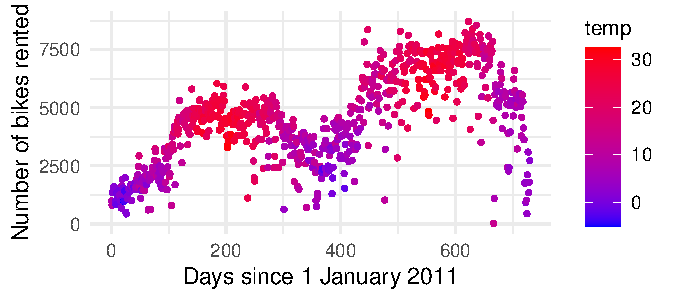
\includegraphics[width=\textwidth]{figures/trend_plot.pdf}
		%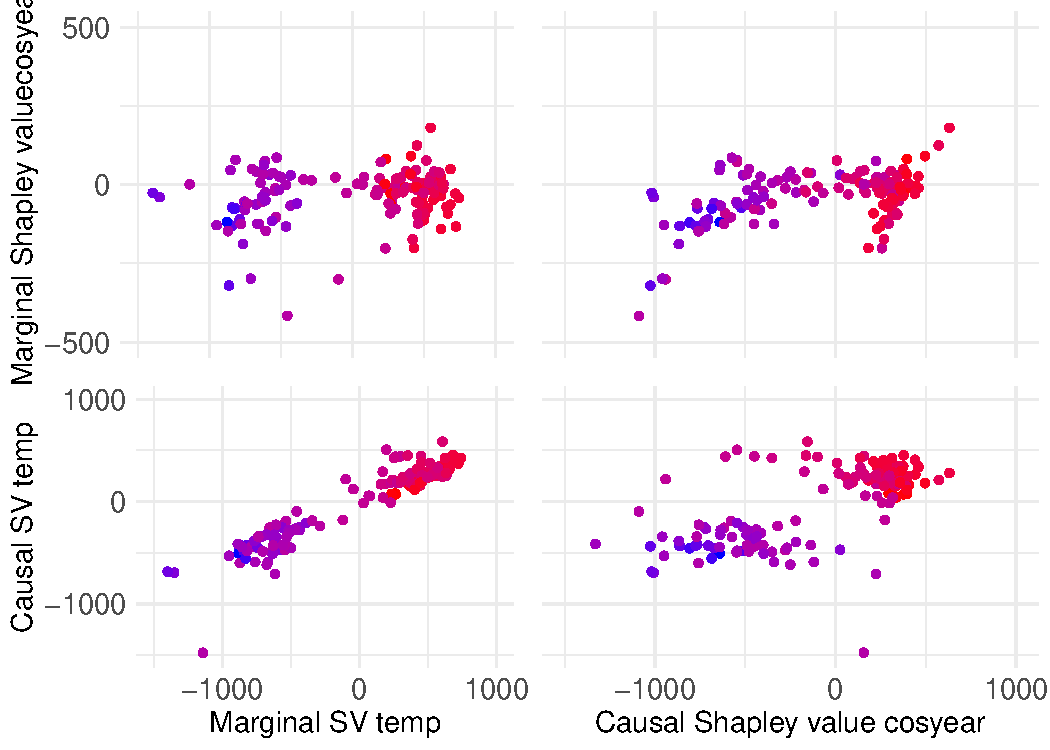
\includegraphics[width=\textwidth]{corr_plots.pdf}
		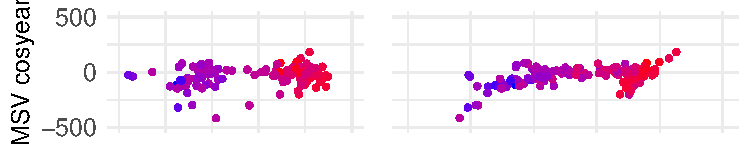
\includegraphics[width=\textwidth]{figures/corr_plots_top.pdf}
		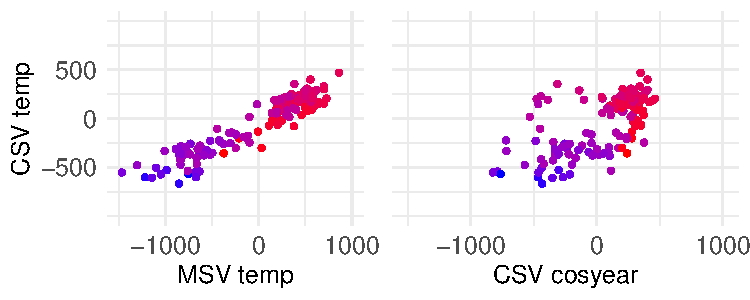
\includegraphics[width=\textwidth]{figures/corr_plots_bottom.pdf}
	\end{minipage}
	\begin{minipage}{.5\linewidth}
		\vfill
		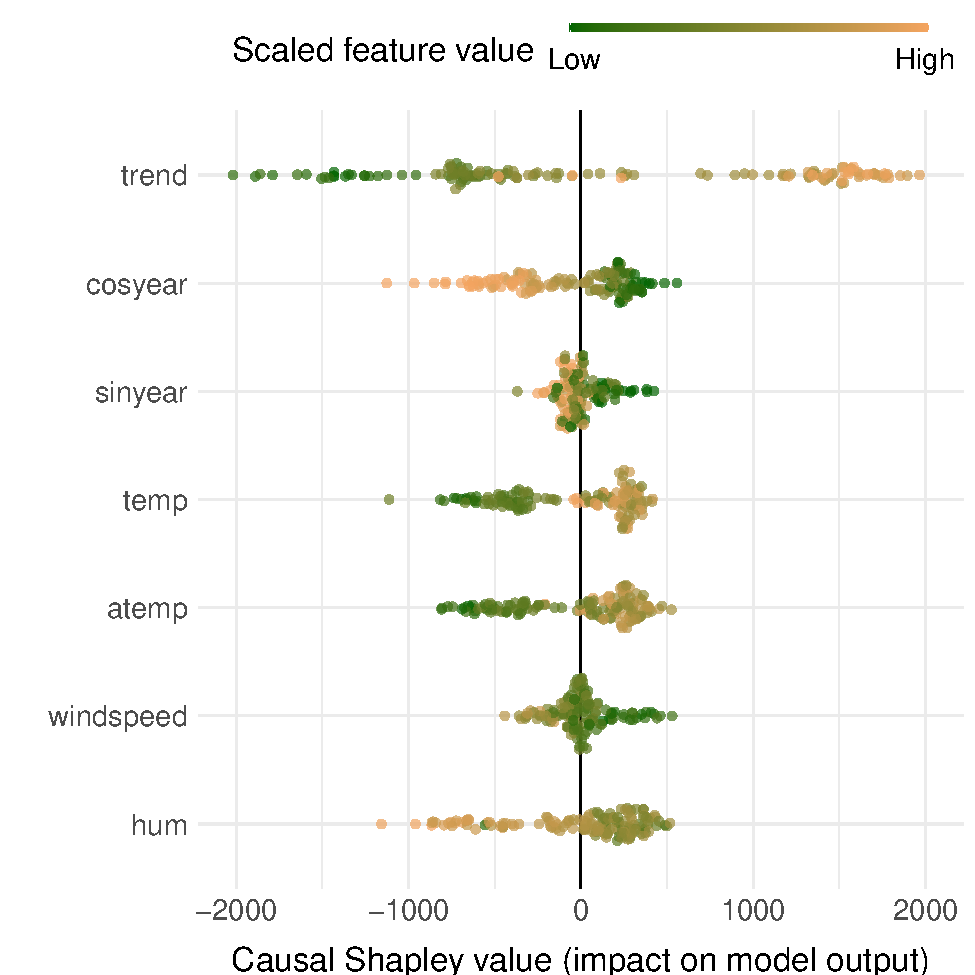
\includegraphics[width=\textwidth]{figures/sina_plot.pdf}
	\end{minipage}
	\caption{Bike shares in Washington, D.C.\ in 2011-2012 (top left; colorbar with temperature in degrees Celcius). Sina plot of causal Shapley values for a trained XGBoost model, where the top three date-related variables are considered to be a potential cause of the four weather-related variables (right). Scatter plots of marginal (MSV) versus causal Shapley values (CSV) for temperature ({\em temp}) and one of the seasonal variables ({\em cosyear}) show that MSVs almost purely explain the predictions based on temperature, whereas CSVs also give credit to season (bottom left).}
	\label{fig:trendplot}
\end{figure}

To illustrate the difference between marginal and causal Shapley values, we consider the bike rental dataset from~\cite{fanaee2013bikerental}, where we take as features the number of days since January 2011 ({\em trend}), two cyclical variables to represent season ({\em cosyear}, {\em sinyear}), the temperature ({\em temp}), feeling temperature ({\em atemp}), windspeed ({\em windspeed}), and humidity ({\em hum}). As can be seen from the time series itself (top left plot in Figure~\ref{fig:trendplot}), the bike rental is strongly seasonal and shows an upward trend. Data was randomly split in 80\% training and 20\% test set. We trained an XGBoost model for 100 rounds. 

We adapted the R package SHAPR from~\cite{aas2019explaining} to compute causal Shapley values, which essentially boiled down to an adaptation of the sampling procedure so that it draws samples from the interventional conditional distribution~(\ref{eq:chaininterventional}) instead of from a conventional observational conditional distribution. The sina plot on the righthand side of Figure~\ref{fig:trendplot} shows the causal Shapley values calculated for the trained XGBoost model on the test data. For this simulation, we chose the partial order $(\{\textit{trend}\},\{\textit{cosyear},\textit{sinyear}\},\{\textrm{all weather variables}\})$, with confounding for the second component and no confounding for the third, to represent that season has an effect on weather, but that we have no clue how to represent the intricate relations between the various weather variables. The sina plot clearly shows the relevance of the trend and the season (in particular cosine of the year, which is -1 on January 1 and +1 on July 1). The scatter plots on the left zoom in on the causal (CSV) and marginal Shapley values (MSV) for {\em cosyear} and {\em temp.} The marginal Shapley values for {\em cosyear} vary over a much smaller range than the causal Shapley values for {\em cosyear}, and vice versa for the Shapley values for {\em temp}: where the marginal Shapley values explain the predictions predominantly based on temperature, the causal Shapley values give season much more credit for the higher bike rental in summer and the lower bike rental in winter. A sina plot for the marginal Shapley values, a.o., can be found in the supplement.

\begin{wrapfigure}[20]{r}{0.5\textwidth}
	\begin{center}
		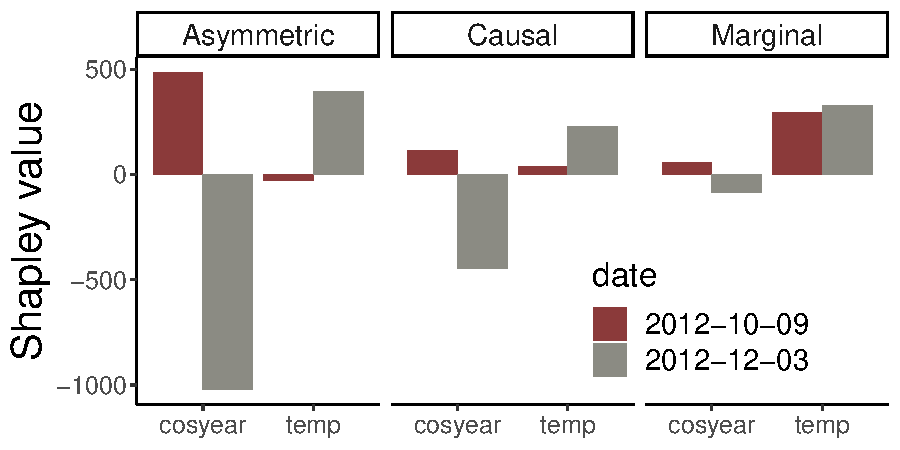
\includegraphics[width=0.48\textwidth]{figures/bar_plots.pdf}
	\end{center}
	\caption{Causal and marginal Shapley values for two different days, one in October (brown) and one in December (gray) with more or less the same temperature of 13 degrees Celsius. Causal Shapley values blame and credit temperature for the relatively low and high predicted bike shares, where marginal Shapley values stay largely indifferent.}
	\label{fig:barplots}
\end{wrapfigure}
The difference between causal and marginal Shapley values possibly becomes even more clear when we consider two days, October 10 and December 3, 2012, with more or less the same temperature of 13 and 13,27 degrees Celsius, and predicted bike counts of 6217 and 6445, respectively. The temperature and predicted bike counts are relatively low for October, yet high for December. The causal and marginal Shapley values for {\em cosyear} and {\em temp} are shown in Figure~\ref{fig:barplots}. The marginal Shapley values provide more or less the same explanation for both days, not really in this case making a distinction between the season and the temperature. The causal Shapley values blame the temperature for the relatively low prediction in October, yet credit the temperature for the relatively high prediction in December, which appears to match human intuition a lot better.

%\comment{To be done: discussion of individual cases, aligned with example in section 3.}


\section{Discussion}

In real-world systems, understanding {\em why} things happen typically implies a causal perspective. It means distinguishing between important, contributing factors and irrelevant side effects. Similarly, understanding why a certain instance leads to a given output by a complex algorithm asks for those features that carry a significant amount of information that contributes to the final outcome. Our insight was to recognize the need to properly account for the underlying causal structure between the features in order to derive meaningful and relevant attributive properties in the context of a complex algorithm.

For that, this paper introduced causal Shapley values, a model-agnostic approach to split a model's prediction of the target variable for an individual data point into contributions of the features that are used as input to the model, where each contribution aims to estimate the total effect of that feature on the target and can be decomposed into a direct and an indirect effect. We contrasted causal Shapley values with (interventional interpretations of) marginal and (asymmetric variants of) conditional Shapley values.
%Conditional and causal Shapley values attribute the difference between a model's prediction for a specific data point and a baseline prediction to the individual features assuming that their values are passively {\em observed} and actively {\em set}, respectively. Both interpretations are valid, but only the latter enables us to leverage additional available information regarding the causal structure. \comment{Rewrite!}
%Marginal Shapley values are perfectly fine when dependencies are purely the result of confounding, as argued in~\cite{janzing2019feature}. However, when these dependencies are the result of causal relationships or even due to selection bias or mutual feedback, then expectations under conditioning by intervention do not simplify to marginal expectations.
We proposed a novel algorithm to compute these causal Shapley values, based on causal chain graphs. All that a practitioner needs to provide is a partial causal order (as for asymmetric Shapley values) and a way to interpret dependencies between features that are on an equal footing.
%Conditioning by intervention becomes conditioning by observation, but only on ancestors and possibly, depending on the interpretation, on features within the same component.
Existing code for computing conditional Shapley values is easily generalized to causal Shapley values, without additional computational complexity. Computing conditional and causal Shapley values can be considerably more expensive than computing marginal Shapley values due to the need to sample from conditional instead of marginal distributions, even when integrated with computationally efficient approaches such as KernelSHAP~\cite{lundberg2017unified} and TreeExplainer~\cite{lundberg2020local}.

Our approach should be a promising step in providing clear and intuitive explanations for output/decisions by a wide variety of complex algorithms, that fits well with natural human understanding and expectations. Additional user studies should confirm to what extent explanations provided by causal Shapley values align with the needs and requirements of practitioners in real-world settings. Similar ideas may also be applied to improve current approaches for (interactive) counterfactual explanations~\cite{wachter2017counterfactual} and properly distinguish between direct and total effects of features on a model's prediction.
If successful, causal approaches that better match human intuition may help to build much needed trust in the decisions and recommendations of powerful modern-day algorithms. 
%where outputs currently often remain underused due to a lack of transparency. Ultimately our goal is to reduce or remove the need to rely on straightforward but sub-optimal ML machinery, so practitioners no longer need to miss out on the huge potential of powerful new developments in AI. 

%Our analysis may also provide a better understanding of asymmetric Shapley values: for all permutations that are consistent with the causal ordering, conditioning by intervention boils down to conditioning by observation. However, the current definition in~\cite{frye2019asymmetric} implicitly assumes that dependencies between features that are on an equal footing is due to mutual feedback, not common confounding. Whether or not to only consider permutations that match the causal ordering depends on the application and possibly one's preference. This paper shows that it is unnecessary to forgo symmetry in order to arrive at a causal interpretation of Shapley values. Roughly speaking, asymmetric (causal/conditioning) Shapley values attribute all indirect effects of a causal variable through a mediator on the output to the causal variable \comment{(is this the right term?)}, subtracting them from the Shapley value of the mediator. Symmetric Shapley values are more conservative and attribute only half to the causal variable.

%There is no single accepted theory explaining how humans attribute effects to potential causes~\cite{icard2017normality}. This makes it impossible to come up with a single explanation approach that works well for all cases, let alone for all users. Understanding the limitations of an approach and conveying those limitations
%
%Much also depends on the interpretation of variables involved (internal or external, )
%Since humans have different ways to attribute effects to potential causes, 
%
%there is no single accepted theory on how humans attribute effects to potential causes, 


%We considered the typical situation in which the examples provided in the training set are purely observational and a machine learning model has learned to represent $\expectation[Y|\vx]$. To provide a sensible causal explanation, we then need to assume that all features are actual causes of the target values. Future research may consider cases in which some of the features are causes of the target variable and others mere consequences, possibly combined with active scenarios in which feature vectors are actively generated and input to an oracle to obtain the corresponding target variable.

%As we have argued in this paper, in comparison with marginal and conditional Shapley values, causal Shapley values better match with how humans attribute possible causes to an effect and lead to more intuitive explanations. User studies should explore to what extent explanations provided by causal Shapley values align with the needs and requirements of practitioners in real-world settings. Causal Shapley values aim to incorporate the causal relationships between the input features, but, like the other Shapley values, treat the prediction model as just an arbitrary function of these input features. That is, there is no need for an underlying assumption that the features are actually causes of the target variable that the prediction model relates to in the actual world. An example, could be a model predicting the probability of a disease with as input features potential causes, such as a genetic predisposition, as well as consequences of the disease, such as test outcomes. Causal Shapley values will still correctly incorporate the causal relationships between the features, but explanations should be interpreted with care: they now only relate to the model predicting the disease, not to the actual disease.



%\comment{Discuss non-manipulable causes as in~\cite{pearl2018obesity}?}
%
%\comment{Compare with counterfactual explanations?}

\section*{Broader Impact}

%Authors are required to include a statement of the broader impact of their work, including its ethical aspects and future societal consequences. 
%Authors should discuss both positive and negative outcomes, if any. For instance, authors should discuss a) 
%who may benefit from this research, b) who may be put at disadvantage from this research, c) what are the consequences of failure of the system, and d) whether the task/method leverages
%biases in the data. If authors believe this is not applicable to them, authors can simply state this.

%Use unnumbered first level headings for this section, which should go at the end of the paper. {\bf Note that this section does not count towards the eight pages of content that are allowed.}

%\begin{ack}
%Use unnumbered first level headings for the acknowledgments. All acknowledgments
%go at the end of the paper before the list of references. Moreover, you are required to declare 
%funding (financial activities supporting the submitted work) and competing interests (related financial activities outside the submitted work). 
%More information about this disclosure can be found at: \url{https://neurips.cc/Conferences/2020/PaperInformation/FundingDisclosure}.

Our research, which aims to provide an explanation for complex machine learning models that can be understood by humans, falls within the scope of explainable AI (XAI). XAI methods like ours can help to open up the infamous ``black box'' of complicated machine learning models like deep neural networks and decision tree ensembles. A better understanding of the predictions generated by such models may provide higher trust~\cite{ribeiro2016should}, detect flaws and biases~\cite{kusner2017counterfactual}, higher accuracy~\cite{bhatt2020explainable}, and even address the legal ``right for an explanation'' as formulated in the GDPR~\cite{gdpr2017}.

Despite their good intentions, explanation methods do come with associated risks. Almost by definition, any sensible explanation of a complex machine learning system involves some simplification and hence must sacrifice some accuracy. It is important to better understand what these limitations are~\cite{kumar2020problems}. Model-agnostic general purpose explanation tools are often applied without properly understanding their limitations and over-trusted~\cite{kaur2020interpreting} They could possibly even be misused just to check a mark in internal or external audits. Automated explanations can further give an unjust sense of transparency, sometimes referred to as the `transparency fallacy'~\cite{edwards2017slave}: overestimating one's actual understanding of the system. Last but not least, tools for explainable AI are still mostly used as an internal resource by engineers and developers to identify and reconcile errors~\cite{bhatt2020explainable}.

Causality is essential to understanding any process and system, including complex machine learning models. Humans have a strong tendency to reason about their environment and to frame explanations in causal terms~\cite{sloman2005causal,lombrozo2017causal} and causal-model theories fit well to how humans, for example, classify objects~\cite{rehder2003causal}. In that sense, explanation approaches like ours, that appeal to a human's capability for causal reasoning should represent a step in the right direction~\cite{mittelstadt2019explaining}.


\bibliography{shapleyrefs}
\bibliographystyle{plain}



\end{document}
